%%%%%%%%%%%%%%%%%%%%%%%%%%%%%%%%%%%%%%%%%
% kaobook
% LaTeX Class
% Version 0.9.8 (2021/08/23)
%
% This template originates from:
% https://www.LaTeXTemplates.com
%
% For the latest template development version and to make contributions:
% https://github.com/fmarotta/kaobook
%
% Authors:
% Federico Marotta (federicomarotta@mail.com)
% Based on the doctoral thesis of Ken Arroyo Ohori (https://3d.bk.tudelft.nl/ken/en)
% and on the Tufte-LaTeX class.
% Modified for LaTeX Templates by Vel (vel@latextemplates.com)
%
% License:
% LPPL (see included MANIFEST.md file)
%
%%%%%%%%%%%%%%%%%%%%%%%%%%%%%%%%%%%%%%%%%

%----------------------------------------------------------------------------------------
%	EXAMPLE AND DOCUMENTATION OF THE KAOBOOK CLASS
%----------------------------------------------------------------------------------------

\documentclass[
    letterpaper, % Page size
    fontsize=10pt, % Base font size
    twoside=false, % Use different layouts for even and odd pages (in particular, if twoside=true, the margin column will be always on the outside)
	%open=any, % If twoside=true, uncomment this to force new chapters to start on any page, not only on right (odd) pages
	%chapterentrydots=true, % Uncomment to output dots from the chapter name to the page number in the table of contents
	numbers=noenddot, % Comment to output dots after chapter numbers; the most common values for this option are: enddot, noenddot and auto (see the KOMAScript documentation for an in-depth explanation)
]{kaobook}

%----------------------------------------------------------------------------------------
%	PACKAGES AND OTHER DOCUMENT CONFIGURATIONS
%----------------------------------------------------------------------------------------

% Choose the language
\ifxetexorluatex
	\usepackage{polyglossia}
	\setmainlanguage{english}
\else
	\usepackage[english]{babel} % Load characters and hyphenation
\fi
\usepackage[english=british]{csquotes}	% English quotes

% Load packages for testing
\usepackage{blindtext} % Print text without any meaning for testing purposes
%\usepackage{showframe} % Uncomment to show boxes around the text area, margin, header and footer
%\usepackage{showlabels} % Uncomment to output the content of \label commands to the document where they are used

% Load the bibliography package
\usepackage{kaobiblio}
\addbibresource{main.bib} % Bibliography file

% Load mathematical packages for theorems and related environments
\usepackage[framed=true]{kaotheorems}

% Load the package for hyperreferences
\usepackage{kaorefs}
\graphicspath{{examples/documentation/images/}{images/}} % Paths in which to look for images

\makeindex[columns=3, title=Alphabetical Index, intoc] % Make LaTeX produce the files required to compile the index

\makeglossaries % Make LaTeX produce the files required to compile the glossary
\newglossaryentry{computer}{
	name=computer,
	description={is a programmable machine that receives input, stores and manipulates data, and provides output in a useful format}
}

% Glossary entries (used in text with e.g. \acrfull{fpsLabel} or \acrshort{fpsLabel})
\newacronym[longplural={Frames per Second}]{fpsLabel}{FPS}{Frame per Second}
\newacronym[longplural={Tables of Contents}]{tocLabel}{TOC}{Table of Contents}

 % Include the glossary definitions

\makenomenclature % Make LaTeX produce the files required to compile the nomenclature

% Reset sidenote counter at chapters
%\counterwithin*{sidenote}{chapter}

%----------------------------------------------------------------------------------------

\begin{document}


%----------------------------------------------------------------------------------------
%       FRONT COVER
%----------------------------------------------------------------------------------------

% If you have a PDF/image file that you want to use as a back cover, uncomment the following lines

%\clearpage
%\thispagestyle{empty}
%\null
%\clearpage
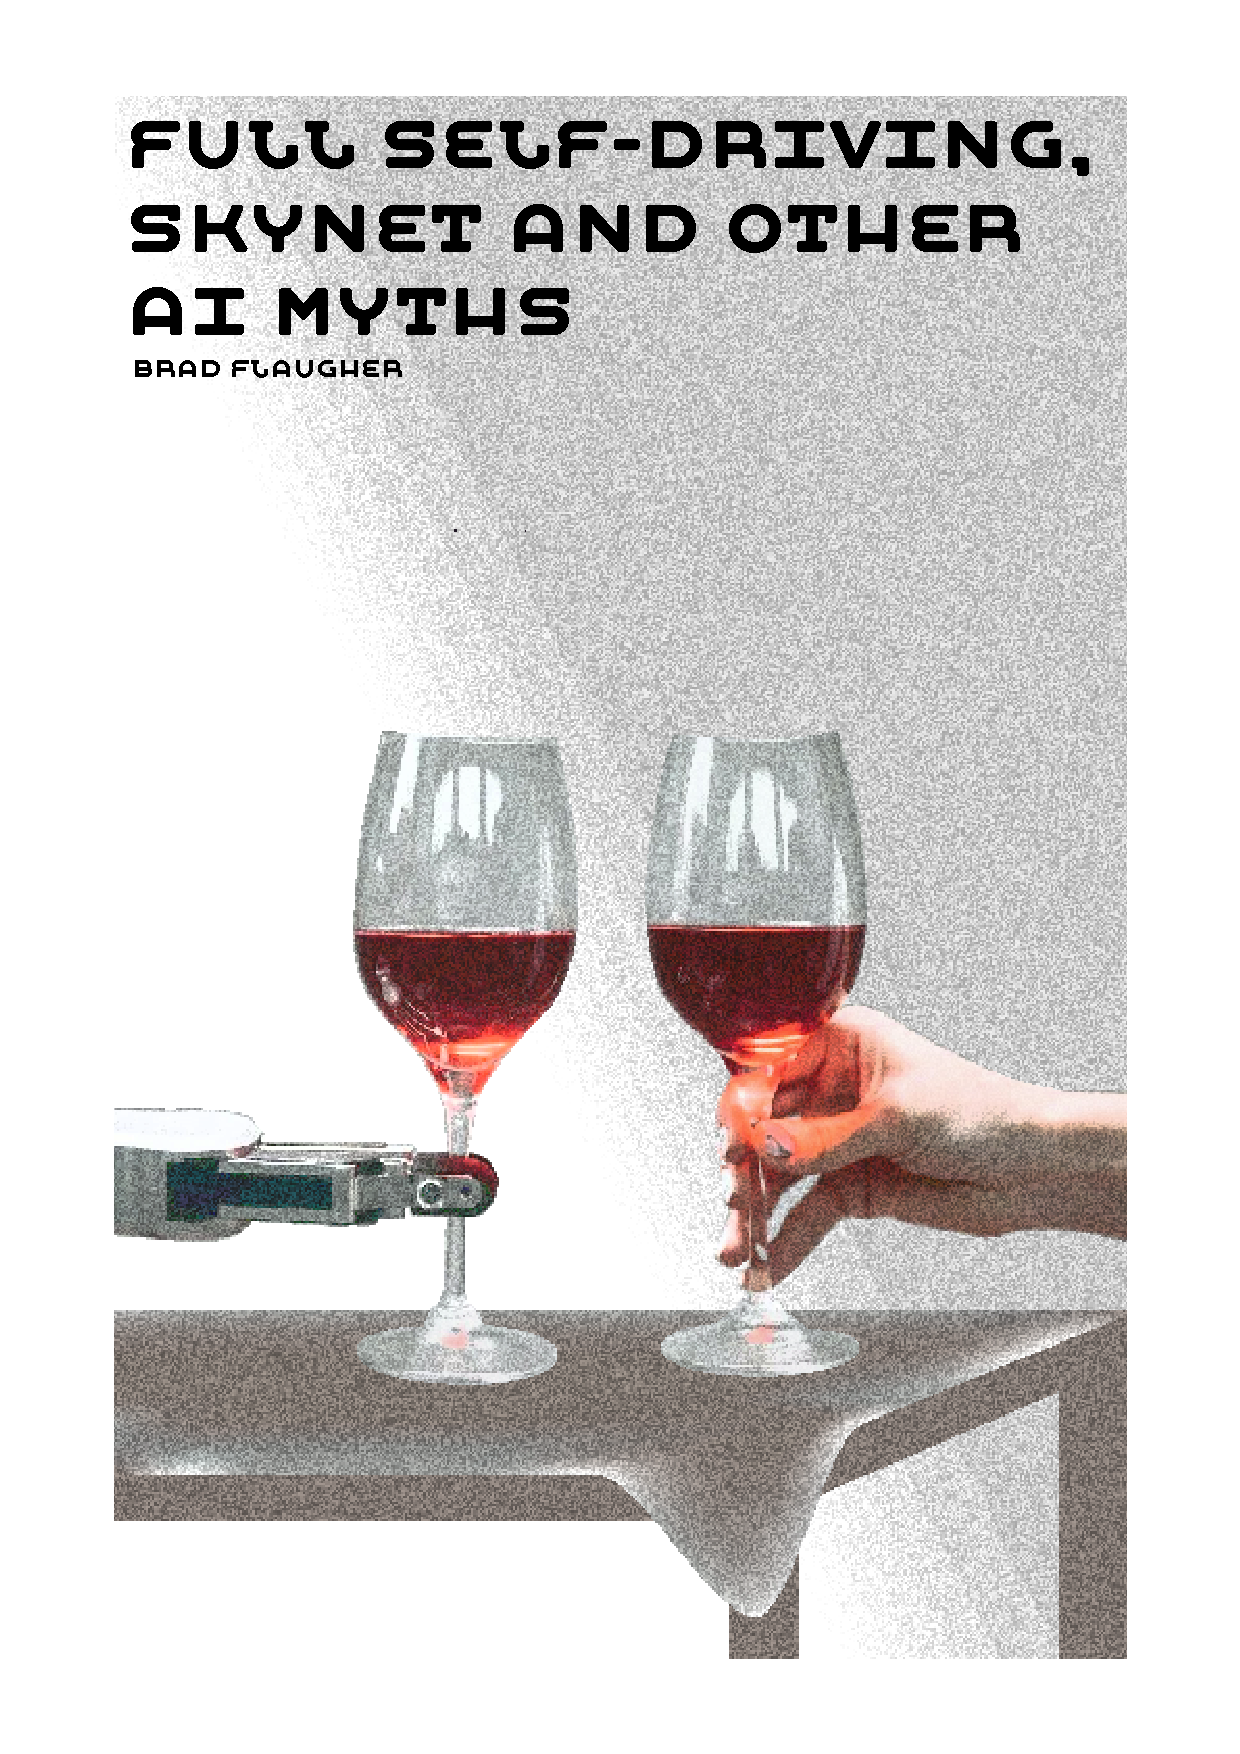
\includepdf{cover.pdf}

%----------------------------------------------------------------------------------------


%----------------------------------------------------------------------------------------
%	BOOK INFORMATION
%----------------------------------------------------------------------------------------


\title[ Full Self-Driving, Skynet and other Artificial Intelligence Myths ]{ Full Self-Driving, Skynet and Other Artificial Intelligence Myths }
\subtitle{ Modern decision making with deep machine learning models }

\author[Brad Flaugher]{Brad Flaugher}

\date{\today}

\publishers{}

%----------------------------------------------------------------------------------------

\frontmatter % Denotes the start of the pre-document content, uses roman numerals

%----------------------------------------------------------------------------------------
%	OPENING PAGE
%----------------------------------------------------------------------------------------

%\makeatletter
%\extratitle{
%	% In the title page, the title is vspaced by 9.5\baselineskip
%	\vspace*{9\baselineskip}
%	\vspace*{\parskip}
%	\begin{center}
%		% In the title page, \huge is set after the komafont for title
%		\usekomafont{title}\huge\@title
%	\end{center}
%}
%\makeatother

%----------------------------------------------------------------------------------------
%	COPYRIGHT PAGE
%----------------------------------------------------------------------------------------

\makeatletter
\uppertitleback{\@titlehead} % Header

\lowertitleback{
	\textbf{Disclaimer}\\
	You can edit this page to suit your needs. For instance, here we have a no copyright statement, a colophon and some other information. This page is based on the corresponding page of Ken Arroyo Ohori's thesis, with minimal changes.
	
	\medskip
	
	\textbf{No copyright}\\
	\cczero\ This book is released into the public domain using the CC0 code. To the extent possible under law, I waive all copyright and related or neighbouring rights to this work.
	
	To view a copy of the CC0 code, visit: \\\url{http://creativecommons.org/publicdomain/zero/1.0/}
	
	\medskip
	
	\textbf{Colophon} \\
	This document was typeset with the help of \href{https://sourceforge.net/projects/koma-script/}{\KOMAScript} and \href{https://www.latex-project.org/}{\LaTeX} using the \href{https://github.com/fmarotta/kaobook/}{kaobook} class.
	
	The source code of this book is available at:\\\url{https://github.com/fmarotta/kaobook}
	
	(You are welcome to contribute!)
	
	\medskip
	
	\textbf{Publisher} \\
	First printed in May 2019 by \@publishers
}
\makeatother

%----------------------------------------------------------------------------------------
%	DEDICATION
%----------------------------------------------------------------------------------------

\dedication{
\textit{We have now accumulated sufficient evidence to see that whatever language the central nervous system is using, it is characterized by less logical and arithmetical depth than what we are normally used to.}\\
	-- John von Neumann, 1958 \cite{vonNeumann2012}
}

%----------------------------------------------------------------------------------------
%	OUTPUT TITLE PAGE AND PREVIOUS
%----------------------------------------------------------------------------------------

% Note that \maketitle outputs the pages before here

\maketitle

%----------------------------------------------------------------------------------------
%	PREFACE
%----------------------------------------------------------------------------------------

\chapter*{Preface}
\addcontentsline{toc}{chapter}{Preface} % Add the preface to the table of contents as a chapter

This book is a work in progress, I hope it helps demystify the world of deep learning as I understand it.

Humans won't be able to control superintelligent AI, talk about that here\cite{Andreu2021}

Talk about Bostrom and GPAI here, and Erdi's answer to that. \cite{Erdi2019} \cite{Bostrom2014}

Talk about the alignment problem and Ethical freakouts about AI. Talk about the big 3 from 
\cite{Christian2020}
\cite{Blackman2022Jul}

Funding and startups, everybody is doing it, I'm trying to make sense of it


\begin{flushright}
	\textit{Brad Flaugher}
\end{flushright}

\index{preface}

%----------------------------------------------------------------------------------------
%	TABLE OF CONTENTS & LIST OF FIGURES/TABLES
%----------------------------------------------------------------------------------------

\begingroup % Local scope for the following commands

% Define the style for the TOC, LOF, and LOT
%\setstretch{1} % Uncomment to modify line spacing in the ToC
%\hypersetup{linkcolor=blue} % Uncomment to set the colour of links in the ToC
\setlength{\textheight}{230\hscale} % Manually adjust the height of the ToC pages

% Turn on compatibility mode for the etoc package
\etocstandarddisplaystyle % "toc display" as if etoc was not loaded
\etocstandardlines % "toc lines as if etoc was not loaded

\tableofcontents % Output the table of contents

% \listoffigures % Output the list of figures

% Comment both of the following lines to have the LOF and the LOT on 
% different pages
% \let\cleardoublepage\bigskip
% \let\clearpage\bigskip

% \listoftables % Output the list of tables

% \listoflstlistings % Output the list of listings

\endgroup

%----------------------------------------------------------------------------------------
%	MAIN BODY
%----------------------------------------------------------------------------------------

\mainmatter % Denotes the start of the main document content, resets page numbering and uses arabic numbers
\setchapterstyle{kao} % Choose the default chapter heading style

\setchapterpreamble[u]{\margintoc}
\chapter{The Artificial Intelligence Industrial Complex}
\labch{introduction}

\textit{"There was a time when everyone thought the quants had figured it out. That is not the perception today. When it comes to the stockmarket, at least, automation has not been the winner-takes-all event that many fear elsewhere. It is more like a tug-of-war between humans and machines. And though the machines are winning, humans have not let go just yet. "} "Lessons from finance's experience with artificial intelligence" The Economist, Mar 9th 2023 \cite{finaieconomist}


\section{The AI Renaissance}

Technology often finds its first adopters among those who can afford it and foresee its potential. Artificial Intelligence (AI) is no exception, with its early applications dating back several decades, notably in the financial industry. Hedge funds and investment banks identified the immense value of AI and started using it for trading and portfolio management.

Renaissance Technologies, a hedge fund founded by mathematician James Simons, exemplifies the early adoption of AI. Since the 1980s, the company has used AI to predict market movements and optimize trading strategies. By employing highly skilled PhDs known as "quants" to develop algorithms and AI models, Renaissance Technologies has become one of the most successful hedge funds in history.

As AI gained traction, tech giants like Google and Microsoft began investing in their own quants. These experts were tasked with using AI to address a wide range of challenges, from refining search algorithms to enhancing language processing capabilities. Much of this research was made public, allowing the broader community to benefit from these advancements.

AI has had a transformative effect on the advertising industry as well. Algorithms now analyze user behavior and target ads with remarkable precision. This has led to an increased demand for privacy-conscious products and services. For example, I carry a Faraday cage fanny pack from a company called "Mission Darkness" to avoid being tracked when I don't want to be. It's a modern-day solution for shielding against unwanted surveillance and data collection.

The accessibility of AI technology has increased, thanks in part to open-source projects that enable individuals and smaller organizations to tap into its power. This democratization of AI has ignited a wave of innovation, with developers worldwide contributing to the AI renaissance.

However, the ubiquity of AI raises some pressing concerns. In a world where data is valuable, the phrase "information wants to be free" takes on new significance. As AI models become more valuable, the risks of data theft and unauthorized sharing escalate. Companies and individuals are striving to protect their intellectual property while others look for ways to exploit it.

This situation sets the stage for an AI copyright battle looming on the horizon. As the distinction between proprietary and open-source information blurs, the question of who owns AI-generated content becomes increasingly important. Governments, corporations, and individuals are all grappling with the legal and ethical implications of AI and its widespread adoption.

So, the AI renaissance has brought about significant advancements in technology, transforming industries and reshaping our world. From the early days of hedge funds like Renaissance Technologies to the current era of open-source AI projects, the landscape has evolved rapidly. As AI continues to permeate our lives, the challenges of data ownership and privacy will become even more critical. In the coming years, we can expect new AI-powered innovations, but also new debates and conflicts as society grapples with the implications of this powerful technology.

\sidecite{copyrighteconocmist}

\section{AI Shrinks the Market, but Takes 80\% Market Share}

The "Software Paradox" posits that as software becomes more valuable, it tends to shrink markets while capturing most of the market share. This phenomenon can be observed in the current state of AI, particularly with the advent of open-source AI. As AI technologies become more sophisticated and widespread, they are reducing the need for human labor in many markets, while simultaneously capturing a significant portion of the market share.\sidecite{OGrady2015}

One key aspect of AI's impact on the market is its ability to automate repetitive and mundane tasks, allowing humans to focus on more complex and creative aspects of their work. This not only streamlines processes but also has the potential to improve the overall quality of work. With AI handling the less desirable tasks, human workers can concentrate on utilizing their unique skills and expertise, resulting in better outcomes and higher value-added work.

The rise of open-source AI further accelerates this trend, making advanced AI tools and algorithms accessible to a broader range of individuals and organizations. As these powerful tools become more widely available, businesses across various industries will find it increasingly difficult to justify the cost of employing human workers for tasks that can be more efficiently completed by AI. This shift will result in a smaller job market for those specific tasks, with AI taking the majority of the market share.

However, the shrinking of specific labor markets does not necessarily mean the eradication of all human work. Instead, it presents an opportunity for the workforce to adapt and focus on roles that are complementary to AI systems. This could involve tasks that require empathy, complex problem-solving, or human intuition, which are areas where AI currently struggles to excel.

\section{The Other Economy, the One Without AI}

As AI revolutionizes various sectors of the economy, there's another economy that remains untouched by AI's transformative effects. This other economy is characterized by heavily regulated industries that often resist technological innovation, resulting in stagnating growth and rising costs for consumers\sidecite{andreesenunemp}.

In many places, AI is practically illegal. This is partly due to consumers, professional organizations and governments struggling to keep up with the rapid pace of technological advancements, leading to a lack of understanding and appropriate regulations \sidecite{lawmakersny}. Additionally, public opinion remains skeptical about the widespread adoption of AI, as evidenced by polls\sidecite{morningconsult}\sidecite{monmouthai}. This skepticism is not helped by stories of software developers becoming emotionally attached to AI chatbots\sidecite{googlenerd}.

The contrast between sectors that embrace AI and those that resist it highlights a growing divide in the economy. In industries where AI is allowed to flourish, technological innovation drives down prices and increases product quality, leading to a more efficient market. However, heavily regulated sectors that resist AI adoption experience rising costs and stagnating growth, ultimately consuming a larger share of the economy.

This phenomenon is exacerbated by the emotional interplay between production and consumption. As consumers, we tend to become frustrated with price increases in the heavily regulated sectors. On the other hand, as producers, we may feel threatened by technological disruption in industries that embrace AI. This dichotomy demonstrates the inherent conflict between the desire for stability in the economy and the need for innovation and progress.

As the regulated, non-technological sectors continue to grow as a percentage of GDP, the economy may ultimately become dominated by these stagnating industries. In such a scenario, the full potential of AI and other advanced technologies may never be realized. This highlights the importance of addressing regulatory barriers, fostering public understanding, and promoting AI adoption in industries that have yet to embrace its potential.

The existence of an economy without AI underscores the challenges that lie ahead in integrating advanced technologies into every aspect of our lives. To fully realize the benefits of AI, it is crucial to address the legal, regulatory, and public perception barriers that currently hinder its adoption. By doing so, we can work towards a more efficient and innovative economy that harnesses the power of AI for the benefit of all.


\section{(Human and AI) Workers of The World, Unite!}

AI's adoption can be seen as an extension of the outsourcing trend that has been prevalent for decades. The principle "if you can't beat them, join them" seems more relevant than ever, as people increasingly integrate AI into their work and lives.

Even in places where AI is technically illegal or frowned upon, individuals find creative ways to leverage AI to make their lives easier. Students may use AI to help write essays, office workers may employ Optical Character Recognition (OCR) to avoid tedious data entry tasks, and programmers might utilize GitHub Copilot regardless of whether their employers approve. These examples demonstrate that as AI tools become more accessible and affordable, they will infiltrate various industries.

\begin{marginfigure}[-5.5cm]
    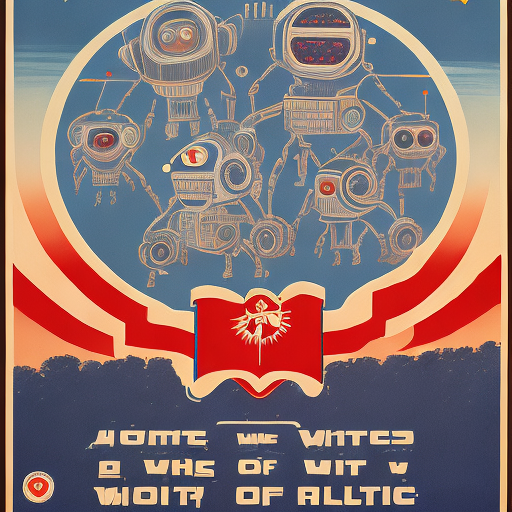
\includegraphics{unite}
        \caption{"mdjrny-v4 style a propaganda poster that says 'AI and Human Workers of the World Unite' featuring some robots and humans laboring together in the fields, USSR-style 8k" made with Mann-E}
        \labfig{marginunite}
\end{marginfigure}

Instead of resisting this trend, we should work with it and guide its development. Embracing AI and integrating it into our work processes can lead to increased productivity, innovation, and overall improvement in our quality of life\sidecite{peopleusingAIhappy}.

The situation with AI usage is reminiscent of self-driving cars and semi-autonomous driving modes. Despite manufacturers' intentions and guidelines, these features are often treated as fully autonomous by users, reflecting the human tendency to push boundaries and adapt technology to suit their needs.

As AI becomes more ingrained in our daily lives, it's essential to recognize the inevitability of its adoption and focus on guiding its development in a way that maximizes its benefits and minimizes potential risks. By uniting human and AI workers, we can foster a collaborative environment that leverages the strengths of both entities and paves the way for a more efficient, innovative, and prosperous future. \sidecite{protopia}

\section{Is it The Future Yet?}

AI, as a general-purpose technology, has the potential to transform various aspects of our lives. However, its widespread adoption and impact on Total Factor Productivity (TFP) might not happen overnight. History has shown that even groundbreaking general-purpose technologies can take time to reach their full potential.

Take electricity, for example. Although Thomas Edison invented the light bulb in 1879, it took several decades for electricity to become the primary power source in industries and households. The infrastructure required to generate and distribute electricity on a large scale was built gradually, and businesses needed time to adapt their processes and machinery to leverage this new energy source. It wasn't until the early 20th century that the true impact of electricity on productivity and economic growth was realized.

Another example is the steam engine, invented by James Watt in 1775, which marked the beginning of the Industrial Revolution. The technology's full potential was not realized until several decades later. The adoption of steam-powered machinery required significant investments in infrastructure and the reorganization of production processes. Additionally, the development of railway networks and steamships expanded the reach of this technology, leading to a profound impact on productivity and global trade.

The internet also followed a similar pattern. While the internet was conceived in the late 1960s, it wasn't until the 1990s that its commercial potential began to be explored. The widespread adoption of the internet required the development of user-friendly web browsers, the expansion of telecommunications infrastructure, and the emergence of e-commerce platforms. It took several years for the internet to become an integral part of our daily lives and contribute to increased productivity across various industries.

So, while AI has the potential to revolutionize numerous aspects of our lives, it may take time for this technology to fully permeate our society and yield its maximum benefits. Patience and continuous innovation will be essential in realizing the transformative potential of AI. By learning from the history of general-purpose technologies, we can better understand the trajectory AI might follow and work towards a future where it significantly impacts productivity and our everyday lives.

\section{Key Takeaways}

\begin{itemize}
    \item \textbf{Deep learning presents challenges and opportunities}, with the potential to become a powerful, free tool for innovation.\sidenote{The Free Software Foundation's goals align with the inherent nature of deep learning models.}
    \item \textbf{Deep learning can be used as an "employee"} for non-critical tasks, offering a balance between dystopian and utopian visions of the future.\sidenote{Work will transform, and humans will act as supervisors and managers of these new technological workers.}
\end{itemize}
  
\setchapterpreamble[u]{\margintoc}
\chapter{The Regression Theory of Everything}
\labch{regression}

\textit{"AI Scientists disagree as to whether these language networks possess true knowledge or are just mimicking humans by remembering the statistics of millions of words. I don't believe any kind of deep learning network will achieve the goal of AGI [Artificial General Intelligence] if the network doesn't model the world the way the brain does. Deep learning networks work well, but not because they solved the knowledge representation problem. They work well because they avoided it completely, relying on statistics and lots of data instead. How deep learning networks work is clever, their performance impressive, and they are commercially valuable. I am only pointing out that they don't possess knowledge and, therefore, are not on the path to having the ability of a five-year-old child."} Jeff Hawkins, 2022 \cite{hawkins2022}

\section{Let's Avoid Knowledge Representation!}

The knowledge representation problem in AI is the challenge of how to formally represent knowledge in a way that a computer can understand and reason about. This typically involves creating a set of symbols, rules, and structures that can be used to represent concepts, relationships, and other types of information. The goal is to create a representation that is both expressive enough to capture all relevant aspects of the domain, and computationally tractable enough to allow for efficient reasoning and inference. There are many different approaches to knowledge representation, including logic-based, semantic networks, frames, and ontologies, each with their own strengths and weaknesses.

Deep learning techniques handle knowledge representation differently than traditional symbolic AI methods. Unlike symbolic AI, which relies on explicit and hand-coded representations of knowledge, deep learning techniques learn to represent knowledge implicitly through the use of neural networks.


\begin{marginfigure}[-5.5cm]
        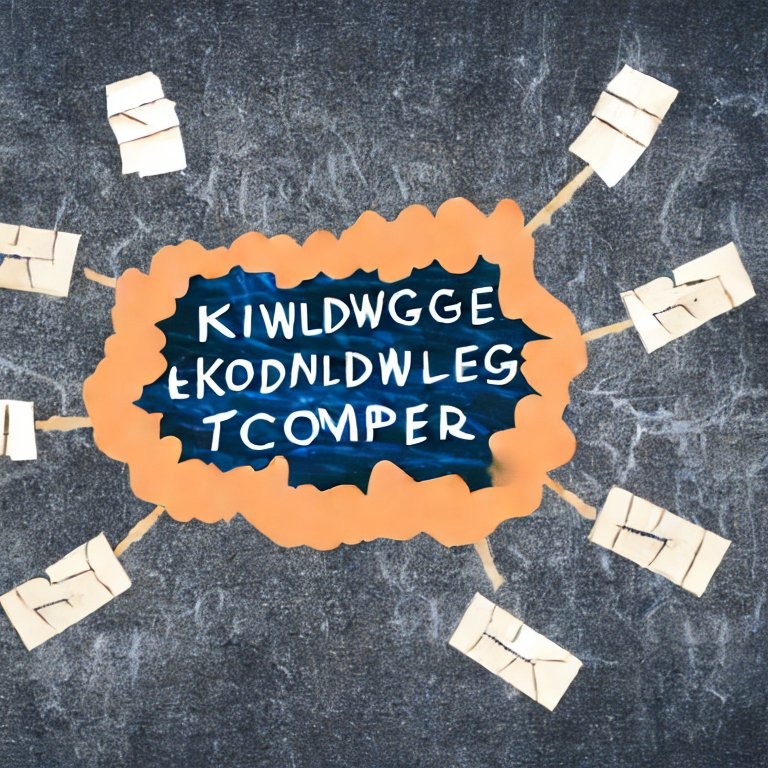
\includegraphics{knowledge}
        \caption{"mdjrny-v4 a disembodied computer being force-fed data like a duck looking somewhat like a sci-fi character 8k" made with Mann-E}
        \labfig{marginknowledge}
\end{marginfigure}


In deep learning, knowledge is represented in the form of the weights of the neural network. These weights are learned through training on a large dataset and they capture the underlying relationships and patterns in the data. The neural network can then use these learned weights to make predictions, classifications or generate new data.

Deep learning models can handle large and complex datasets, and can automatically extract features from the data without the need for manual feature engineering. This makes them particularly well-suited for tasks such as image and speech recognition, natural language processing, and other areas where large amounts of data are available. However, they are not as good at explicating how they arrived at a decision, which can be a disadvantage.

In summary, deep learning techniques handle knowledge representation by learning the underlying patterns and relationships in the data through the use of neural networks, which can then be used for prediction, classification, and generation tasks. In GOFAI, knowledge is held by the programmer and explicitly coded into rules, deep learning methods instead use data to guess the best rules from the relationships peresent in the dataset. 

\section{A Simple Neural Network is also a Linear Regression}

A neural network can be mathematically equivalent to a regression or a decision tree under certain conditions.

A neural network is a machine learning model composed of layers of interconnected artificial neurons, which are designed to process and analyze data. They can be used for a wide range of tasks, such as image and speech recognition, natural language processing, and prediction.

\begin{marginfigure}[-5.5cm]
	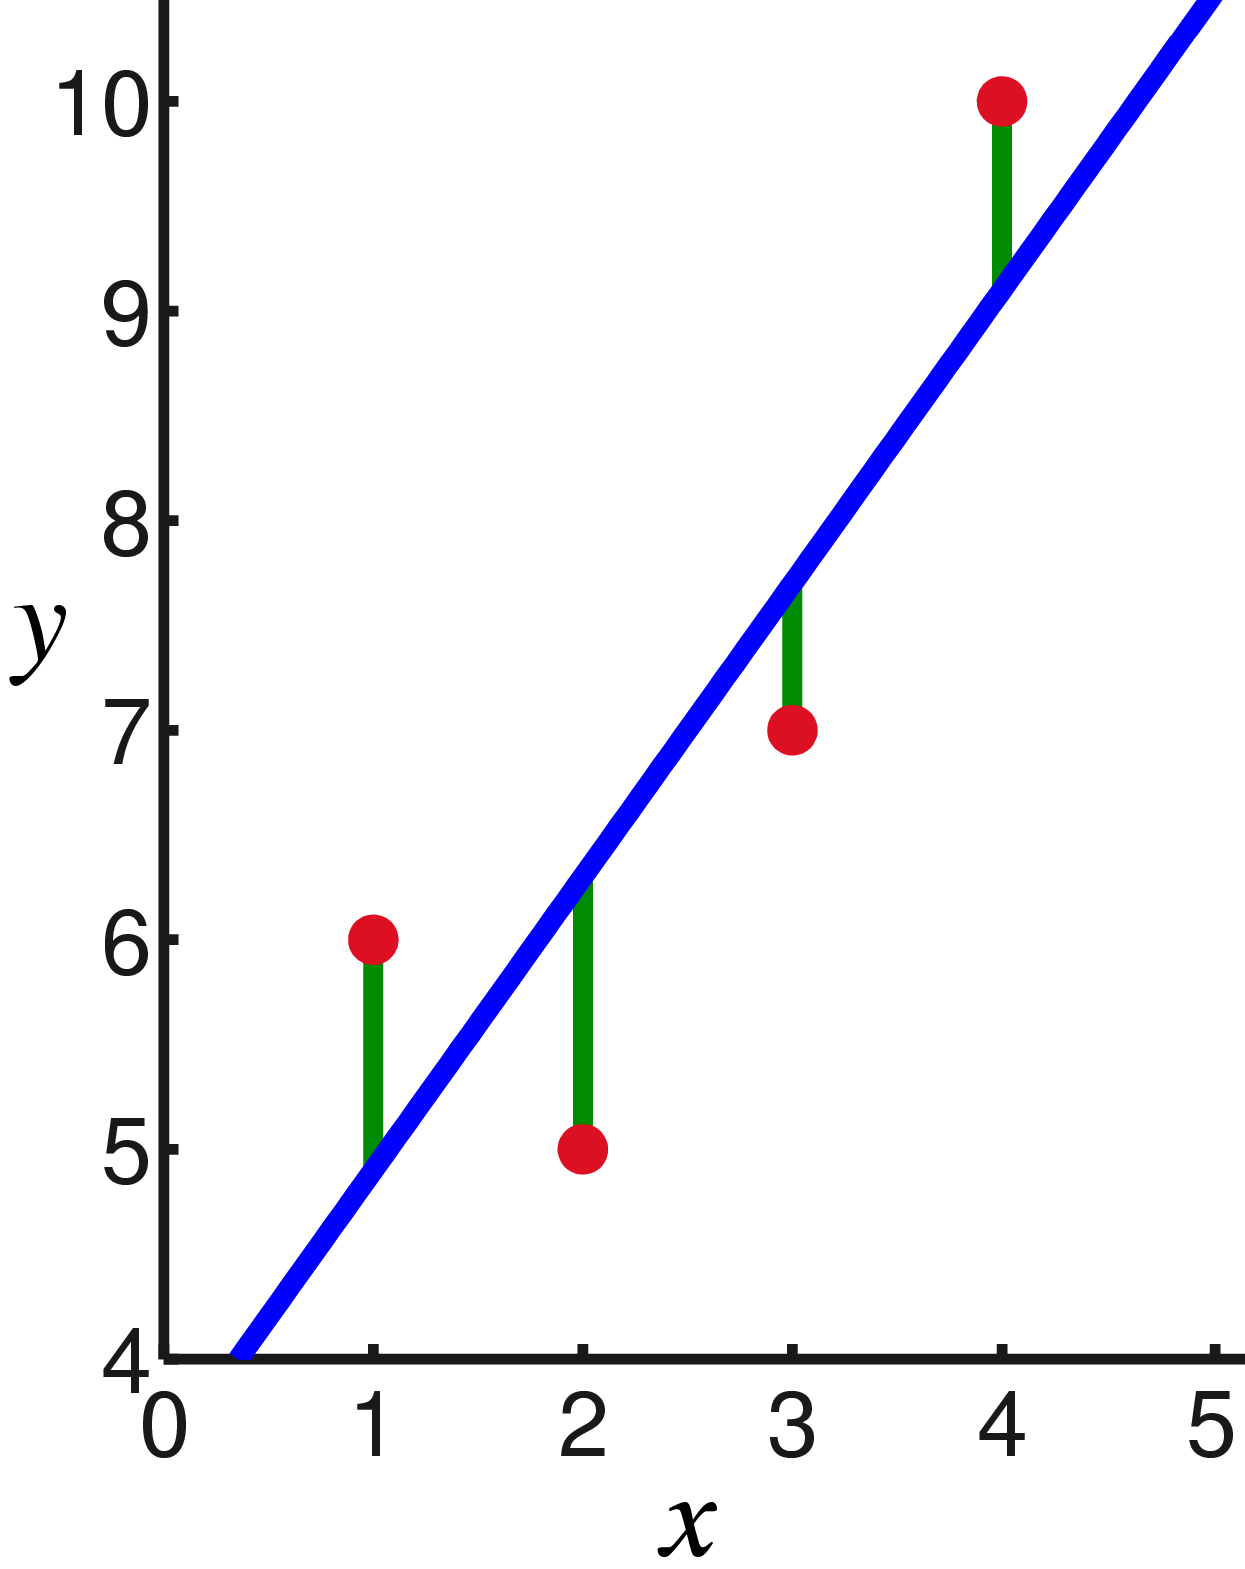
\includegraphics{OLSregression}
        \caption{A simple linear regression, the red points are the training data, and the blue line is the regression line. If you don't understand this please read \url{https://en.wikipedia.org/wiki/Regression_analysis}}
        \labfig{olsregression}
\end{marginfigure}


A regression is a statistical method used to predict a continuous variable based on one or more input features. A linear regression, for example, is a simple neural network with one input layer, one output layer and no hidden layers. In this case, the weights of the network are the coefficients of the linear equation and the network is equivalent to a linear regression model.

A decision tree is a tree-based model used for classification and prediction tasks. It consists of a series of if-then rules that are used to make decisions based on the input data. A neural network with one input layer, one output layer and one hidden layer\sidenote{One with a ReLU activation, Neurons in a neural network can have different activation functions, if you don't know what it is and don't want to read about it on wikipedia, that's OK. \url{https://en.wikipedia.org/wiki/Activation\_function}} is equivalent to a decision tree. The network implements a piecewise linear function which can represent the decision boundaries of a decision tree. So, under certain conditions, a neural network can be mathematically equivalent to a linear regression or a decision tree. These conditions include having one input and one output layers, and having a specific activation function in the case of a decision tree.\sidecite{Aytekin}

\section{Dummy Variables for Dummies (Wonkish)} 

Chapter Summary: It's all numbers, man. Machine learning techniques require that we turn everything (images, text, sound) into numbers and shove them into the model in the same way we use dummy variables in a simple regression. If you are satisfied with this, please skip this section. If you would like to learn a bit about the details and see some code examples, please keep reading. This section is necessarily technical, but should be approachable for anyone who has taken a college statistics class. \sidenote{Thanks to Paul Krugman for popularizing (to me at least) the \textit{wonkish} classifier, I just mean it's a little nerdy. But it's important.} 



Dummy variables are used in regression analysis to include categorical variables in a model. Categorical variables are variables that take on a finite number of distinct values, such as "red", "green", "blue" or "yes", "no". Since these variables cannot be directly included in a regression model, as they are not numerical, they need to be transformed into numerical variables.

The process of creating dummy variables is also known as one-hot encoding. It involves creating a new binary variable for each category of the original variable. For example, if you have a categorical variable "color" with three categories: "red", "green", "blue", you would create three binary variables: "color\_red", "color\_green", "color\_blue". Each binary variable would take a value of 1 if the original variable is equal to the category, and 0 otherwise.

When using dummy variables in a regression, it is important to remember to include only n-1 binary variables, where n is the number of categories in the original variable. This is because including all n binary variables would result in perfect multicollinearity, which is when two or more independent variables are perfectly correlated. One of the binary variables can be dropped to avoid this problem.

Dummy variables are used in regression analysis to include categorical variables in a model. The process of creating dummy variables involves creating a new binary variable for each category of the original variable and one-hot encoding it. It is important to remember to include only n-1 binary variables, to avoid perfect multicollinearity.



\begin{marginlisting}[-0.5cm]
\caption{Mapping text to numbers.}
\vspace{0.2cm}
\begin{lstlisting}[language=Python,style=kaolstplain]
 'movies': 99,
 'after': 100,
 'think': 101,
 'characters': 102,
 'watch': 103,
 'two': 104,
 'films': 105,
 'character': 106,
 'seen': 107,
 'many': 108,
 'being': 109
\end{lstlisting}
\end{marginlisting}


The creation of dummy variables in a regression is analogous to preprocessing image, text and other data for a neural network for deep learning. This preprocessing is important  as it ensures that the data is in a format that can be easily understood and processed by the network. The preprocessing steps for numbers, text, and images are slightly different.

For numbers:
\begin{itemize}
	\item Normalization: It is common to normalize the input data by scaling it to have a mean of 0 and a standard deviation of 1. This helps to ensure that all input features have similar scales and prevents any one feature from dominating the network's computations.
	\item Imputation: Handling missing data is important, as it can negatively impact the model's performance. Common imputation techniques include replacing missing values with the mean, median, or mode of the feature.
\end{itemize}

For text:

\begin{itemize}
	\item Tokenization: Text data must first be converted into a numerical format that can be understood by the network. This is typically done by tokenizing the text into individual words or n-grams and then encoding them as integers or real-valued vectors. A one-hot encoding exactly like the dummy variable method used in regression is also frequently used. \sidenote{Sometimes text is just mapped to a number! Shocking, but it works. See how it is taught in the TensorFlow tutorials \url{https://www.tensorflow.org/text/guide/word\_embeddings}} \sidenote{GPT-3 uses byte-level Byte Pair Encoding (BPE) tokenization and has a vocabulary size of 50,257.}
	\item Stop-words removal: The most common words in any language like "a", "an", "the", etc. that do not contain much meaning are called stop-words, they are often removed to reduce the dimensionality of the data.
	\item Stemming/Lemmatization: Words that have the same meaning can be stemmed or lemmatized to reduce the vocabulary size and increase the chances of generalization.
	\item Vocabulary Size: Each model must choose a vocabulary size or the maximum number of tokens that it will analyze. This may cause misspellings, slang or typos to be discarded in analysis.
\end{itemize}

For images:
    
\begin{itemize}
	\item Converting to RGB or Greyscale: Each image is analyzed by its pixel color value, every point on an image will either have 3 color values (red, green, blue) or one single value (on a white/black scale) if the image is analyzed in greyscale.
	\item Convolutions\sidenote{If you would prefer a visualization of a neural network check out this excellent video by Dennis Dmitriev \url{https://www.youtube.com/watch?v=3JQ3hYko51Y}.}: Pixel values are analyzed in groups that are defined by the model, since individual pixel values are only colors (or greyness) they must be combined together by the model to detect patterns like faces and stop signs. The method of convolution is defined by the model itself.
	\item Resizing: neural network can only accept images of a fixed size, so resizing the image to match the network's requirements is important.
	\item Normalization: It is common to normalize the pixel values to be in the range of 0-1 or -1 to 1. This will help the model converge faster.
	\item Data Augmentation: To increase the amount of data and prevent overfitting, common data augmentation techniques such as flipping, rotation, and cropping can be applied to the images.
\end{itemize}

In summary, preprocessing is an important step in training a neural network, as it ensures that the data is in a format that can be easily understood and processed by the network. The preprocessing steps for numbers, text, and images involve normalization, imputation, tokenization, stop-words removal, stemming/lemmatization, resizing and data augmentation.

\section{Try That Again With A Few Billion Parameters}

In the first section of this chapter we introduced the idea that a simple neural network is mathematically equivalent to a regression. This is true and a useful way to think about neural networks and deep learning. \sidenote{\begin{equation}y=Wx+b\end{equation} There's your simple formula for a single-cell neural network and regression, in practice we'll change $W$, $x$ and $b$ to matrices and introduce nonlinear activation function $f$ so, \begin{equation}y=f(Wx+b)\end{equation} if you please. If equations scare you, don't worry about it for now.} 

In practice, a neural network trained on a gaming PC from 2023 can easily have millons of trainable parameters. A simple image classifier used to classify handwritten digits might have 60,000 parameters which is about the number the model used by Yann LeCun and company in the 1990s. Bleeding-edge deep neural networks are trained on large GPU farms and have have billions of trainable parameters. More parameters gives the models tremendous power to recognize complex patterns, but also makes any practical attempt at explaining their inner-workings impossible.  

\begin{marginfigure}[-5.5cm]
        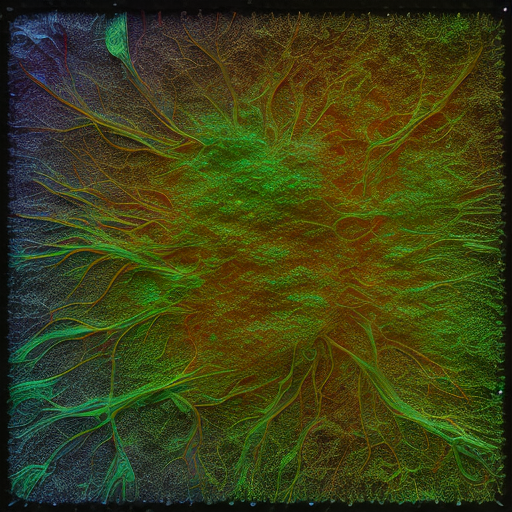
\includegraphics{greenneuron}
        \caption{"mdjrny-v4 layers and layers of neurons looking like a gooey lasagna, but the data has green blood 8k" made with Mann-E}
        \labfig{marginneuron}
\end{marginfigure}


When a neural network has millions of trainable parameters and deep layers of neurons\sidenote{In case you are wondering, the human brain has about 86 billion neurons that do the "thinking". Physical neurons are more complicated than the neurons used in deep learning and have supporting structures like astrocytes that do some computation as well. \url{https://en.wikipedia.org/wiki/Astrocyte}}, it can be difficult to explain to a human what each of those parameters represents or how they contribute to the overall function of the network. This is because the interactions between the different layers and neurons can be complex and non-linear, making it challenging to understand the specific role of each parameter. The parameters  model complex interactions between the inputs, making it difficult to understand their specific function. Furthermore, in deep neural networks, the high number of layers can lead to high level of abstraction, meaning that the individual neurons and their weights have little interpretability.

When a neural network has millions of interacting parameters, it can lead to mathematical chaos \sidenote{Mathematical chaos is a real thing, it refers to the behavior of certain dynamic systems that are highly sensitive to initial conditions. This sensitivity leads to seemingly random and unpredictable behavior, even though the underlying equations governing the system are deterministic (meaning they are transparent and known to us). \url{https://en.wikipedia.org/wiki/Chaos_theory} }, which is a phenomenon where small changes in the initial conditions of the network can lead to vastly different outputs. This is because the interactions between the large number of parameters can create non-linear relationships that are sensitive to small changes. This can make it difficult to predict the behavior of the network, as small changes in the input or the parameters can lead to unexpected and seemingly random outputs.\sidenote{Chaotic outputs in a large deterministic system are OK in many domains, and there are controls that can be put in place to keep AI "safe" but deep learning by itself will not produce those controls.}

\section{Multicolinearity and the End of Science}
\labsec{multi}

Data science is a horrible term because it implies that data scientists are scientists and that the work they do is scientific when in reality data scientists are not scientists and the work they do is not scientific. Data scientists use mathematics, statistics, and computer science to analyze data, but it is not scientific in the traditional sense. Data scientists do not use the scientific method and do not conduct experiments or develop theories. Data science is more akin to engineering or data analytics than actual scientific research.

The main goal of a scientist is to gain knowledge and understanding of the natural world through research, experimentation, and data analysis. Scientists make models of the world to test and explain. So-called data scientists make models too but a model with layers of interacting parameters, trained under chaotic conditions is almost impossible to explain. Multicolinearity\sidenote{"Multicolinearity is when two or more variables in a study are closely related to each other. Think of it like dating: imagine you are trying to figure out what makes someone a good partner. You might look at things like how much they make, how attractive they are, and how kind they are. But, these things are all related to each other. For example, attractive people might make more money, and kind people might be more attractive. So, it's hard to know which one is really important for being a good partner, because they are all related. That's like multicolinearity in a study." By ChatGPT given the prompt "explain multicolinearity to a teenager using a dating example"} is just one issue, but deep learning techniques are practically incompatible with the scientific method. With deep learning methods it can be difficult to determine which variable had the most impact on the outcome of the model. Coefficients of the model to be unstable and unreliable, which can make it difficult to explain the model in a meaningful way. 

Explaining the inner-workings of a neural network with millions of interacting parameters is difficult for many reasons. Most of the complexity is due to the number of parameters, which can make it difficult to understand how the model works and why it makes certain decisions. The interactions between the parameters are often non-linear and can be difficult to understand, as the model can be sensitive to small changes in the parameters, which is the definition of mathematical chaos. This can make it difficult to explain why the model is making certain decisions, as the interactions between the parameters are not always clear.

\section{Let's Test Some Random Inputs! Feature Importance and Explainability}
\labsec{explain}

With a huge complex system of neurons that combine inputs in novel ways, it becomes vary hard to understand which inputs are the most important for the system as a whole. To better understand deep learning models, data scientists use randomized or averaged inputs to a model to test the feature importance of a deep learning neural network. This type of testing is done to determine which features are most influential in the overall output of the network. This is done by randomly or averaging the input values for each feature and then running the model to see how the output is affected. For example, if a neural network is used to detect objects in an image, the data scientist may randomize the color of the objects to see how the model’s accuracy is affected. If the accuracy drops significantly, they can infer that color is an important feature in the network.

Randomized or averaged inputs to a model can also be used to determine if a particular feature is necessary for the network to function correctly. For example, if the output of the network is not as accurate when a particular feature is randomized or averaged, then the data scientist can infer that this feature is important for the network’s performance. By using this method, data scientists can gain insights into which features are important and which can be removed from the model to improve performance.

\section{The Universal Machine Learning Workflow}
\labsec{limits}

The Universal Machine Learning Workflow\sidecite{chollet2022} is an important chapter in a technical guide for data scientists  by the author of the most popular machine learning framework in the world\sidenote{It's called TensorFlow and was one of the most popular and "Most Loved" Technologies of 2022 \url{https://survey.stackoverflow.co/2022/\#most-popular-technologies-misc-tech}} that outlines the \textit{Universal} workflow for machine learning projects. I think this chapter should be understood by everyone using, investing in and creating machine learning models. 

Before Chollet gets into the details of model building, he chooses to begin with a note on ethics: 

\textit{"You may sometimes be offered ethically dubious projects, such as “building an AI that rates the trustworthiness of someone from a picture of their face.” First of all, the validity of the project is in doubt: it isn’t clear why trustworthiness would be reflected on someone’s face. Second, such a task opens the door to all kinds of ethical problems. Collecting a dataset for this task would amount to recording the biases and prejudices of the people who label the pictures. The models you would train on such data would merely encode these same biases into a black-box algorithm that would give them a thin veneer of legitimacy. In a largely tech-illiterate society like ours, “the AI algorithm said this person cannot be trusted” strangely appears to carry more weight and objectivity than “John Smith said this person cannot be trusted,” despite the former being a learned approximation of the latter. Your model would be laundering and operationalizing at scale the worst aspects of human judgement, with negative effects on the lives of real people.}

\begin{marginfigure}[-5.5cm]
        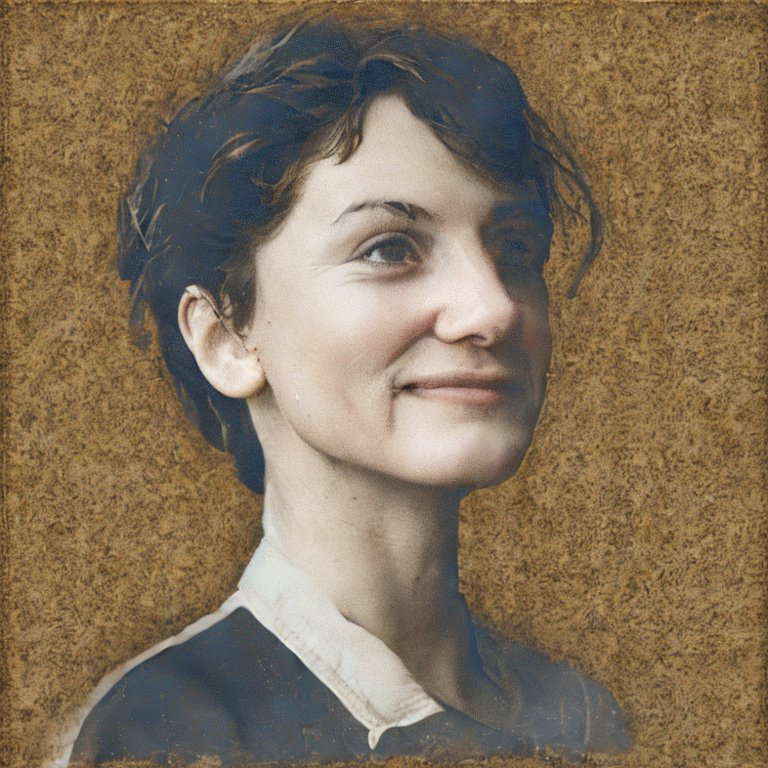
\includegraphics{trustworthysd}
        \caption{"the face of a trustworthy person" made with Stable Diffusion 2.1. (Hey, it's a white lady!)}
        \labfig{trustworthysd}
\end{marginfigure}

\textit{Technology is never neutral. If your work has any impact on the world, this impact has a moral direction: technical choices are also ethical choices. Always be deliberate about the values you want your work to support."}\cite{chollet2022}

Chollet uses the outline below to explain the \textit{Universal} workflow. I'll summarize the workflow and my own notes for a nontechnical audience here:
\begin{enumerate}
    \item Define the Task 
    \begin{enumerate}
        \item Collect a Dataset \sidenote{This is often the hardest part. Data is often labeled by hand or stolen from another domain. See \url{https://en.wikipedia.org/wiki/Transfer_learning}}
        \item Understand Your Data 
        \item Choose a Measure of Success \sidenote{Accuracy isn't everything! We might prefer a less accurate model that avoids false-positives in some scenarios.} 
    \end{enumerate}
    \item Develop a Model
    \begin{enumerate}
        \item Prepare the Data \sidenote{This is discussed in section 2.3 above, everything gets turned into numbers.}
        \item Choose an Evaluation Protocol
        \item Beat a Baseline \sidenote{Does your model predict better than a totally random model and/or coin-flip?}
        \item Develop a model that overfits 
        \item Regularize and Tune Your Model
    \end{enumerate}
    \item Deploy the Model
    \begin{enumerate}
        \item Explain Your Work to Your Stakeholders and Set Expectations
\sidenote{This is almost never done. And as Chollet explains this is both difficult and requires mutual understanding and domain knowledge from the part of "the business" and the Machine Learning Engineer.}
        \item Ship an Inference Model
        \item Monitor Your Model in the Wild
        \item Maintain Your Model
    \end{enumerate}
\end{enumerate}

Of all of the steps in the workflow, "Defining The Task" and "Explaining The Work To Shareholders and Setting Expectations" are where the most miscommunication occurs. 

In defining the task, machine learning engineers are often given impossible problems to solve, and because they want to keep paying their mortgage they solve another related problem instead and allow stakeholders to jump to their own conclusions. By clearly understanding what a model is predicting and how the data is collected some of this misunderstanding can be avoided.

I will discuss Large Language Models later, but they all do the same thing. They predict the next words in a sentence, just like the keyboard on your iPhone. They come up with amazing text but by fundamentally understanding what they are predicting you gain insight into their limitations. They are also all trained on the text publicly available on the internet, this includes scientific sources, but also fan-fiction and anime, so the idea that a model trained on this data could be relied on to predict anything truthful is preposterous. 

\begin{marginfigure}[-5.5cm]
        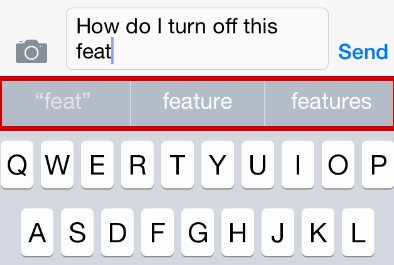
\includegraphics{predictive_keyboard}
        \caption{Fundamentally LLMs are using the same techniques as a predictive keyboard on your phone. This is why Yann Lecun says even though they are impressive some like ChatGPT are not particularly innovative. \url{https://www.youtube.com/watch?v=ULbpPHjiSBg}}
        \labfig{predictivekey}
\end{marginfigure}

Many models work like magic and many users assume models are predicting the future, when they are really correlating based on their past data. Even simple models of creditworthiness might have as similar problem. While building a creditworthiness model for a bank, due to lack of data a machine learning engineer might (on purpose or inadvertently) create a model that predicts whether someone is a smoker instead of whether they are creditworthy. Because smoking and poverty are correlated, maybe the model "works", but it doesn't do what stakeholders think it does. 

Setting expectations is another hellscape of misaligned incentives.\sidenote{The CEO of OpenAI wrote this and still raised ten billion dollars: \textit{"ChatGPT is incredibly limited, but good enough at some things to create a misleading impression of greatness. it's a mistake to be relying on it for anything important right now. it's a preview of progress; we have lots of work to do on robustness and truthfulness."} \url{https://twitter.com/sama/status/1601731295792414720}} Good machine learning engineers and data scientists are supposed to educate and advise stakeholders about the limitations of their own models. Read Chollet's advice on this topic below:

\textit{The expectations of non-specialists towards AI systems are often unrealistic. For example, they might expect that the system "understands" its task and is capable of exercising human-like common sense in the context of the task. To address this, you should consider showing some examples of the failure modes of your model (for instance, show what incorrectly classified samples look like, especially those for which the misclassification seems surprising).} 

\textit{They might also expect human-level performance, especially for processes that were previously handled by people. Most machine learning models, because they are (imperfectly) trained to approximate human-generated labels, do not nearly get there. You should clearly convey model performance expectations. Avoid using abstract statements like "The model has 98 percent accuracy" (which most people mentally round up to 100 percent), and prefer talking, for instance, about false negative rates and false positive rates. You could say, "With these settings, the fraud detection model would have a 5 percent false negative rate and a 2.5 percent false positive rate. Every day, an average of 200 valid transactions would be flagged as fraudulent and sent for manual review, and an average of 14 fraudulent transactions would be missed. An average of 266 fraudulent transactions would be correctly caught." Clearly relate the model's performance metrics to business goals.}


\textit{You should also make sure to discuss with stakeholders the choice of key launch parameters- for instance, the probability threshold at which a transaction should be flagged (different thresholds will produce different false negative and false positive rates). Such decisions involve trade-offs that can only be handled with a deep understanding of the business context.}\cite{chollet2022} 

One does not need to be a psychologist to understand that these conversations almost never happen. The workflow of machine learning is universal, we are all doing fancy regressions and we all deal with the same wild expectations, bad data and misalignment with business.

\begin{marginfigure}[-5.5cm]
        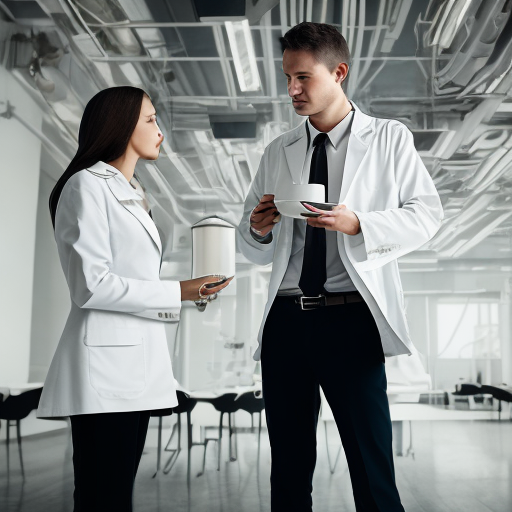
\includegraphics{sciencechat}
        \caption{"mdjrny-v4 a handsome businessperson explaining the business context to a scientist wearing a white coat over coffee 8k" made with Mann-E}
        \labfig{sciencechat}
\end{marginfigure}

\section{A Machine Learning Engineer is a Data Janitor}
\labsec{janitor}

Since the machine learning workflow is \textit{universal}, it is fairly straightforward to automate. There are a plethora of offerings from companies big and small who offer AutoML tools that anyone with basic Excel skills can use\sidenote{See this awesome-AutoML github project for an up-to-date list of commercial AutoML tools \url{https://github.com/windmaple/awesome-AutoML\#commercial-products}}. Since modern AI is "all a regression" these tools do the regression for you, users just need to feed them the data and the AutoML tool finds out the relationship. On the surface it seems like the job of the machine learning engineer has become obsolete before it even became a proper discipline. 

Despite the existence of AutoML tools, machine learning engineers (and data scientists) do some actual work. A 2016\sidenote{I know this study is old, but I have found that the findings still hold when talking to data scientists and/or machine learning engineers that I train and employ.} Crowd Flower survey of 16,000 data scientists showed that on average we spend our time doing the following:

\begin{itemize}
    \item \textbf{60 percent of a machine learning engineer's time is spent cleaning and organizing data}, we are data janitors! If you had great data ready in an Excel file you would have been able to fit your own model without us. We need to organize the mess of data that exists in the world so it is in a nice format to be fit in a model. For example it is well known that almost all large language models use the same common crawl dataset (\url{https://commoncrawl.org/}), but how it is organized and weighted can change the quality of the outputs dramatically. The organization of the same dataset can lead to the same dataset either producing a nice predictive keyboard or something approaching ChatGPT.  
    \item \textbf{19 percent of a machine learning engineer's time is spent collecting data}, we often start making models without a huge dataset, so data needs to be collected in order to make the first model, and after that first model (to match people for our new dating app, let's say) is deployed we rely on users to provide us with data for future models. Collecting new data is a creative endeavour sometimes, and often involves human effort. Amazon's Mechanical Turk\sidenote{"Getting the right training data was another challenge. ImageNet was a collection of one hundred thousand labeled images that required significant human effort to generate, mostly by grad students and Amazon Mechanical Turk workers." \href{https://arstechnica.com/gadgets/2023/01/the-generative-ai-revolution-has-begun-how-did-we-get-here/}{https://arstechnica.com}} service has been leveraged for this purpose for years, and OpenAI has successfully deployed outsourced talent to solve some of the trickiest problems facing large language models\sidenote{Read more about how OpenAI used Kenyan workers to help label toxic content \url{https://time.com/6247678/openai-chatgpt-kenya-workers/}.}.
    \item \textbf{9 percent of a machine learning engineer's time is spent fitting models}, we need to fit models, there is some art to choosing the right architecture and modeling techniques. An AutoML tool can do this reasonably well too, but considering some fancy training servers cost \$28 per hour or more\sidenote{See the latest pricing from AWS here \url{https://aws.amazon.com/sagemaker/pricing/}}, sometimes it is useful to have an expert guess the best model architecture and save time in training, even if that expert is getting paid \$249,000 yer year\sidenote{See the latest machine learning engineer salaries at levels.fyi \url{https://www.levels.fyi/t/software-engineer/focus/ml-ai}}.
    \item \textbf{4 percent of a machine learning engineer's time is spent refining algorithms} many machine learning engineers spend almost no time doing this. Other researchers (corporate-academic types who write scientific papers) spend a lot of time doing this, it averages out to four percent, but doesn't represent the average day of a machine learning engineer.
\end{itemize}

Overall, the main job of most machine learning engineers is to clean up and collect a ton of data, and then feed that data into the same machine learning model that everyone else is using, and then rinse and repeat.\sidenote{Here is a discussion on reddit asking "When was the last time you wrote a custom neural net?" and supports my understanding of the world \url{https://www.reddit.com/r/MachineLearning/comments/yto34q/d_when_was_the_last_time_you_wrote_a_custom/}} 

\section{Key Takeaways}

\begin{itemize}
    \item \textbf{Deep learning models are fundamentally large unscientific regressions} they are trained to create a function that maps input data to output data.
    \item \textbf{Deep learning models are chaotic systems containing millions of interacting parameters} they are not designed to be explained or created in a way that their weights can be used for scientific analysis. They find reasonable answers and don't care how they get there. Multicolinearity (understanding the relationship of an input and output) and feature importance (understanding which inputs are most important) are only understandable with a high level of statistical error.
    \item \textbf{Small changes in inputs of a deep learning model may dramatically change the outputs} deep learning models are complex deterministic systems that can exhibit chaotic behavior. Their inner workings are functionally unknowable and practically impossible to test.
    \item \textbf{Machine learning engineers spend most of their time collecting and organizing data}, because deep learning models often share common architecture, getting good data to train with is the best thing that an engineer can do to train good models. In practice only a handful of corporate-academic types are experimenting with new and exciting architectures. 
    \item \textbf{Deep learning models can have impressive and useful outputs, but the creators of models should be encouraged to highlight their failures and limitations.} Machine learning engineers might be more keen to highlight failures and limitations if they are encouraged to do so by their users, managers and investors.
\end{itemize}


\setchapterpreamble[u]{\margintoc}
\chapter{Creativity and Decision Making with Deep Learning Models}
\labch{intro}

\textit{"AI Policy}

\textit{I expect you to use AI (ChatGPT and image generation tools, at a minimum), in this class. In fact, some assignments will require it. Learning to use AI is an emerging skill, and I provide tutorials in Canvas about how to use them. I am happy to meet and help with these tools during office hours or after class}

\textit{Beware of the limits of ChatGPT:}

\begin{itemize}
	\item\textit{If you provide minimum effort prompts, you will get low quality results. You will need to refine you prompts to get good outcomes. This will take work.}
	\item\textit{Don't trust anything it says. If it gives you a number or a fact, assume it is wrong unless you either know the answer or can check in with another source. You will be responsible for any errors or omissions provided by the tool. It works best for topics you understand.}
	\item\textit{AI is a tool, but one that you need to acknowledge using. Please include a paragraph at the end of any assignment that uses AI explaining what you used the AI for and what prompts you used to get the results. Failure to do so is in violation of academic honesty policies}
	\item\textit{Be thoughtful about when this tool is useful. Don't use it if it isn't appropriate for the case or circumstance."}
\end{itemize}

\textit{Dr. Ethan Mollick, 2023 - Syllabus for class at The Wharton School at the University of Pennsylvania}


\section{Theories of Creativity}

Machine learning models use data (from the past) to discover rules and make classifications. Because of the way they are constructed these classifications, suggestions, artworks are by definition derivative or "having parts that originate from another source". I won't get into a philosophical discussion on what the nature of creativity is, but it's worth considering how using deep learning models biases us towards the past, but also could give us insights from other domains. 

\begin{marginfigure}[-5.5cm]
        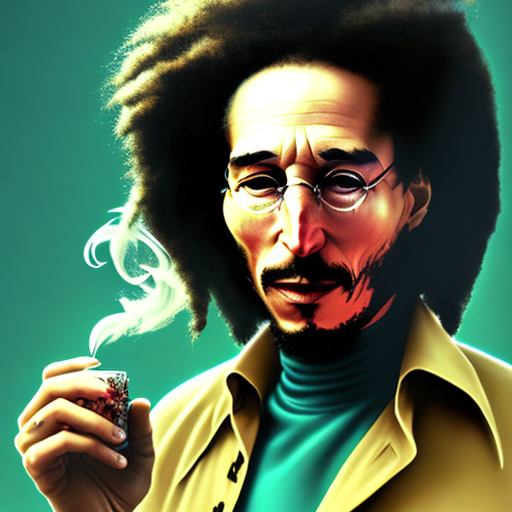
\includegraphics{jobsweed}
        \caption{"mdjrny-v4 Steve Jobs Smoking weed with Bob Marley 8k" made with Mann-E. It's 100\% derivative, but it's art too (I guess).}
        \labfig{jobsweed}
\end{marginfigure}

It can be argued that creativity is simply the combination of existing works. This is because many new ideas and innovations are often inspired by and built upon existing concepts. For example, a new form of music may be created by combining elements from different genres. Similarly, a new technology may be created by combining and improving upon existing technologies.

It can also be argued that creativity involves much more than just combining existing works. Creativity is not just about recombining existing ideas, but also about coming up with completely new and original concepts. This requires a unique perspective and a deep understanding of the subject matter, as well as the ability to think outside the box.  

Deeep learning models of speech, when heavily used, may slow down the evolution of language. AI art models may slow down "progress" in art, whatever that means. Deep learning models of disease trained on data from 1980 may be irrelevant to today's diseases. That said these same models may give us interesting insights in new domains, models trained on beautiful paintings may be put to use in a new domain (like designing beautiful interiors) and that model could give new insight to interior designers, models of the interaction of ants could be put to use in designing cities and so on and so forth. AI cuts many ways, it makes us faster but makes us more reliant on the past, models can be used across domains but should be used intentionally and transparently when possible. Each use opens up a new world of possibilities for users, and sometimes a new headache for intellectual property lawyers. We'll discuss all of these topics in this chapter.

\begin{marginfigure}[-5.5cm]
        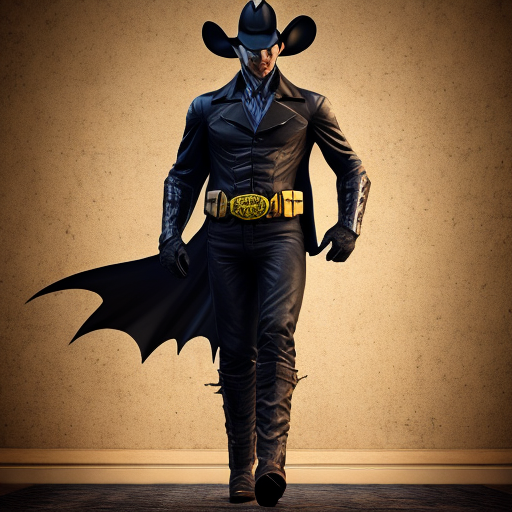
\includegraphics{batman}
        \caption{"Batman dressed as a cowboy" made with Mann-E. It's 100\% derivative as well, but better than any Google image searches I did. It looks amazing! I also might get sued if I use it even though the creators of Mann-E tell me I have the rights to it.}
        \labfig{batman}
\end{marginfigure}

\section{Creative Uses of Power Tools}

Power tools, even simple ones like a drill are complex machines that take human input and transform it using static rules. The pressure the user of a drill puts on the bit and the speed at which they pull the trigger all deterministically affect the output. Just because a tool is a deterministic machine doesn't mean it is unable to produce creative works.

What is happening as we use generative tools like ChatGPT or image-to-text models is that the "creative act" has been relocated. The creative act is now the prompt you give the tool, the users input. And someone can still be good at using AI, just like someone can be good at using any piece of software.

Modern AI is a complex system of algorithms, data, and analytics that can be used to solve complex problems. AI systems can learn from data, identify patterns, and make predictions about the future. AI systems are typically used to automate and assist human decision making. AI systems are programmed with specific objectives and goals, and the user input decides the output. For example, an AI system could be programmed to solve a mathematical problem and the user input would determine the parameters of the problem and the output would be the solution.

A power drill is also a complex deterministic system. The user input is limited to the type of drill bit, the speed of the drill, and the direction of the drill. The output is determined by these inputs, as the drill will only drill in the direction and speed determined by the user. The user also has to choose the correct drill bit to ensure the drill can do the job correctly and safely.

\begin{marginfigure}[-5.5cm]
        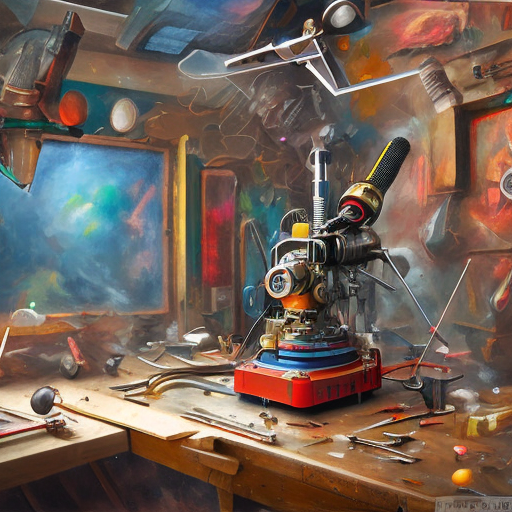
\includegraphics{drillart}
        \caption{"mdjrny-v4 a mikita drill being used in an artist's studio to make a colorful artwork 8k" made with Mann-E}
        \labfig{drillart}
\end{marginfigure}

Both modern deep learning models and a power drill are complex but ultimately deterministic systems. The user input, however limited it may be, ultimately controls the output of the system. Both systems require a user to understand how to use them and to make the correct input to get the desired output.

\section{Garbage In, Garbage Out}

The "Power Tool" of AI is a deterministic, static and unchanging system and the rules of that system are determined by the data that the model is shown. If a model is trained on shitty data, it will produce shitty results. End of book...

... maybe not. It's worth thinking about this for a moment. It is often said that modern AI can "generalize and make informed inferences given new data". If deep learning models are really just a big regression, these models will always come up with an answer, but if the world changes, these models will still be projecting complicated averages of their past data into the future. 

So, let's separate AI's decision making into two extremes; \textit{Creative Decision Making} and \textit{Critical Decision Making}. The stakes are very low in a world of \textit{Creative Decision Making} and who gives a shit if the AI is all a regression, and it just mushes together the limited data that it's seen. In a creative context you can also ask an AI interesting questions, so long as you don't solely rely on it's output without checking the facts first\sidenote{See the syllabus note from Dr. Mollick at the beginning of this chapter.}. Even if "Garbage In, Garbage Out" holds, garbage can still be helpful for a creative process. 

Note that this book is called "Full-Self Driving, Skynet..", a self-driving car and a nuclear-bomb-equipped all-seeing AI are clearly not engaging in any \textit{Creative Decision Making}. 

\section{Garbage In, New Perspective Out?}

For creative tasks, it generally doesn't matter that a deep learning model is unscientific or trained on a lopsided dataset. An informed user of AI knows this and can account for that in their decision making, especially when engaging in creative decision making. The situation becomes problematic once we allow deep learning models to engage in critical decision making by themselves. 

\begin{marginfigure}[-5.5cm]
        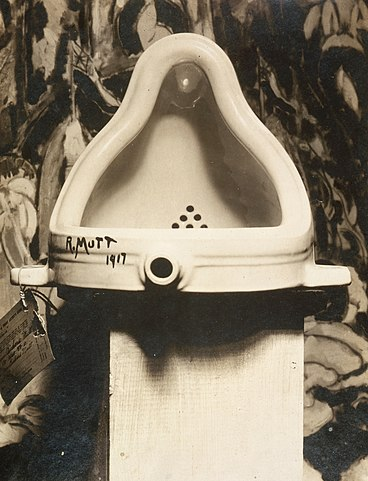
\includegraphics{duchamp}
        \caption{Marcel Duchamp's "Fountain". A urinal that blew peoples minds \url{https://www.tate.org.uk/art/artworks/duchamp-fountain-t07573}.}
        \labfig{duchamp}
\end{marginfigure}

Generative models will come up with amazing (but derivative) works of art, But, they will never "change the game". A model of sculpture trained on past sculptures in 1917 will never come up with Marcel Duchamp's "Fountain". There is a term that machine learning engineers use for this, when the rules of the game are changed, it's called "Concept Drift".

\section{Concept Drift and the End of Usefulness}


Concept drift refers to the phenomenon where the distribution of data changes over time, causing the performance of deep learning models built on historical data to degrade. The model becomes less useful because it is trained to make predictions based on the relationship between the inputs and outputs in the data it was trained on, and if this relationship changes, the model may start making incorrect predictions. This is particularly problematic in real-world applications, where the data is constantly evolving and the relationship between inputs and outputs is subject to change. To mitigate the effects of concept drift, it is often necessary to continually retrain deep learning models on updated data.

The frequency with which a deep learning model needs to be retrained to mitigate the effects of concept drift depends on several factors, including the rate at which the data distribution changes, the size and complexity of the model, and the availability of computational resources.

For some applications with relatively stable data distributions, retraining the model once every few months or even once per year may be sufficient. However, in other applications where the data is changing rapidly, it may be necessary to retrain the model more frequently, such as once per week or even once per day.

\begin{marginfigure}[-5.5cm]
        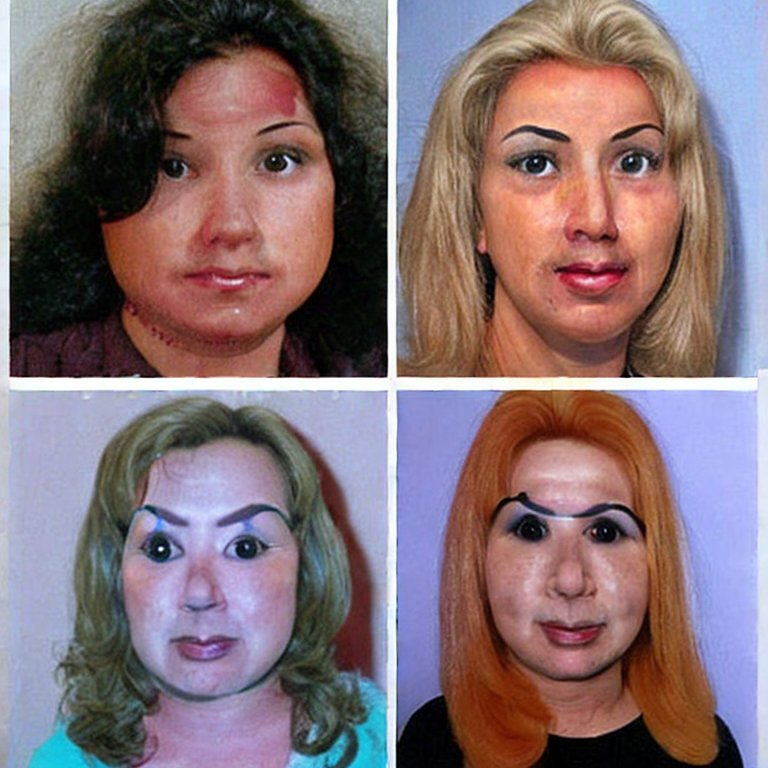
\includegraphics{plastic}
        \caption{"Plastic surgery gone wrong" made with Stable Diffusion. Imagine a model that classifies images as "human face" or "not human face", and imagine that model was trained on images of human faces before 1900, maybe you would not be surprised if you gave it a picture of a human face that had a lot of cosmetic surgery done to it, and that model might say "this is not a human face", the idea of what a human face is has changed over time this is called "concept drift".}
        \labfig{plastic}
\end{marginfigure}

Ultimately, the frequency of retraining will depend on the specific requirements of the application, and the trade-off between the cost of retraining and the potential cost of incorrect predictions. In general, it's recommended to monitor the performance of the model over time and to retrain it as needed to ensure that it remains accurate and relevant.

If a deployed deep learning model is not monitored, there are several risks that can emerge:

\begin{itemize}
\item Accuracy degradation: As the data distribution changes over time, the model may become less accurate, leading to incorrect predictions. This can result in financial losses, reduced customer satisfaction, or even harm to individuals.
\item Bias amplification: deep learning models can be biased, and if this bias is not monitored and addressed, it can be amplified over time as the model continues to make incorrect predictions. This can result in discriminatory outcomes, such as unequal treatment of individuals based on protected characteristics such as race, gender, or age.
\item Legal liability: In some cases, incorrect predictions made by deep learning models can result in legal liability, particularly if the model is being used to make decisions that have significant consequences, such as in the criminal justice system or in medical diagnosis.
\item Reputational damage: If a deep learning model is making incorrect predictions, it can damage the reputation of the organization deploying the model, potentially leading to a loss of customers or investors.
\end{itemize}


It is important to monitor deep learning models once they are deployed, and to take action to address any issues that arise, such as retraining the model or adjusting its parameters, in order to mitigate these risks and ensure that the model continues to perform well over time.

\section{The Impossibility of Fairness}

Achieving fairness in deep learning models can be challenging, and to some extent it may be impossible to completely eliminate all forms of bias. This is because deep learning models are trained on historical data, which may contain biases and disparities that are perpetuated in the model's predictions. One can attempt to "fix the training set" but in practice models will continue to bias their prediction to past data, or their creators careful curation of the past.\sidecite{Christian2020} 

However, it is possible to reduce the impact of bias in deep learning models through careful design and monitoring of the model's performance. This may include techniques such as fairness constraints, algorithmic transparency, and regular auditing of the model's predictions to identify and address any issues of bias.

It's important to note that fairness is a complex and multi-faceted concept, and different definitions of fairness may be appropriate for different applications. For example, some definitions of fairness may prioritize equal treatment of all individuals, while others may prioritize proportional representation or equal opportunities.

Ultimately, the extent to which fairness is achievable in deep learning models will depend on the specific requirements of the application and the level of effort that is put into designing and monitoring the model to ensure that it is making fair and unbiased predictions.

\section{Transfer Learning Everywhere}

Transfer learning is a machine learning technique that involves transferring knowledge from one model trained on a task to another model trained on a related task. The idea behind transfer learning is that a model that has been trained on one task can be fine-tuned for another task, reducing the amount of labeled data required to train the new model.

For example, imagine that you have a deep learning model that has been trained to recognize objects in natural images (cats, dogs, balls, cars). You can use the knowledge learned by this model as a starting point to train a new model that recognizes objects in medical images, such as X-rays or MRI scans. The new model can start with the weights of the pre-trained model and fine-tune them on the new task, using a much smaller amount of labeled data than would be required to train the model from scratch.

Transfer learning can be useful in many different applications, particularly when labeled data is scarce or expensive to obtain. By leveraging knowledge from a pre-trained model, transfer learning can help to improve the performance of new models, reduce the amount of data required for training, and accelerate the development of new machine learning applications.

I asked ChatGPT to "tell me a story of transfer learning going horribly wrong in the context of online dating, with a model trained in the Middle East being deployed by an American dating app." and here's what it said:

\textit{"Once upon a time, an American online dating company decided to use transfer learning to improve their matchmaking algorithms. They trained a state-of-the-art machine learning model on a large dataset of profiles and dating preferences from the Middle East. The model was able to suggest matches with remarkable accuracy and the company was confident that it would perform just as well in the American market.}

\textit{However, things went terribly wrong when they deployed the model on their American dating app. The model was not properly trained to consider the cultural and social differences between the Middle East and America. As a result, it suggested matches that were inappropriate and offensive, causing widespread backlash and criticism from users.}

\textit{For example, the model suggested matches between people of different religious backgrounds, which was not acceptable to many users. It also suggested matches between people with significant age gaps, which was not socially acceptable in the American market.}

\textit{The company was forced to remove the model and start from scratch, causing significant harm to their reputation and financial losses. They learned the hard way that transfer learning can only be effective if the model is properly trained on relevant and culturally appropriate data.}

\textit{This story serves as a cautionary tale about the importance of considering cultural differences and ethical implications when deploying machine learning models in different regions and markets."}

Not bad I think... picking good training data and doing good "data janitoring" is the main job of a machine learning engineer\sidenote{The better your machine learning engineer understands your business problem, the better job they'll do at creating the dataset.}.

If the past is not like the future, you are also doing transfer learning. Most models steal data from other sources so are doing transfer learning too. This is fine, but do we know that we are doing this? A model that is deployed in a domain experiencing concept drift and continues to make predictions without being retrained can be considered to be doing a harmful form of transfer learning. This is because the model has been trained on a different distribution of data (the past), and is being applied to a new domain with a different distribution (the present and future).

In traditional transfer learning, the goal is to transfer knowledge from one domain to another related domain, where the data distributions are similar enough to enable the model to make accurate predictions. However, in the case of concept drift, the data distributions are changing over time, and the model is becoming less accurate as a result. \sidenote{Think about your life and if you "transferred" your model of thinking from when you were 12 years old, to "today" when you are 35 years old, that is a bad model to be operating on! That model needs to be updated. We'll explore many examples of where this is and is not a problem in the next chapter."}

By continuing to make predictions without being retrained, the model is essentially "transferring" its knowledge from a historical data distribution to a new, changed data distribution, which may not be a valid assumption. This can result in incorrect predictions and other negative outcomes, such as harm to individuals or organizations.

\section{Industrial-Scale Plagiarism}

Aside from regurgitating the past and predictions from other domains, deep learning models can also enable plagiarism on an industrial scale. Early text generation models could be made to write entire sections of \textit{Harry Potter} when fed the opening lines of a chapter. Even as models grow large and more sophisticated, users, researchers and lawyers are still able to "extract the training data"  from large models\sidecite{Carlini2023}, causing headaches for their creators and adding to the work of intellectual property lawyers. 

To avoid this creators of deep learning models have the following tools at their disposal:


\begin{itemize}
\item Best practices in  machine learning: data preprocessing, augmentation, reuglarization, model architecture choices, early stopping and validation are all things that we are taught to do to prevent overfitting.
\item Contractual agreements: Microsoft (owner of github and cocreator of the \href{https://github.com/features/copilot}{Github Copilot} code generation model) has a special contract for anyone submitting code to github that essentially says that "we are allowed to use this code to train our models, and if our models regenerate your copyrighted code, you can go fuck yourself."
\item Release the Kraken: StabilityAI's Stable Diffusion model was released as open source software, they still managed to get sued \cite{getty}, but they basically said, "this model was trained on all copyrighted and copylefted images on the web, sometimes it'll generate stuff that violates copyright law, but we are in Germany and will give this thing away for free to the public, and see how Getty Images, photographers and graphic designers of the world handle it... OKbye!". 
\end{itemize}


\begin{marginfigure}[-5.5cm]
        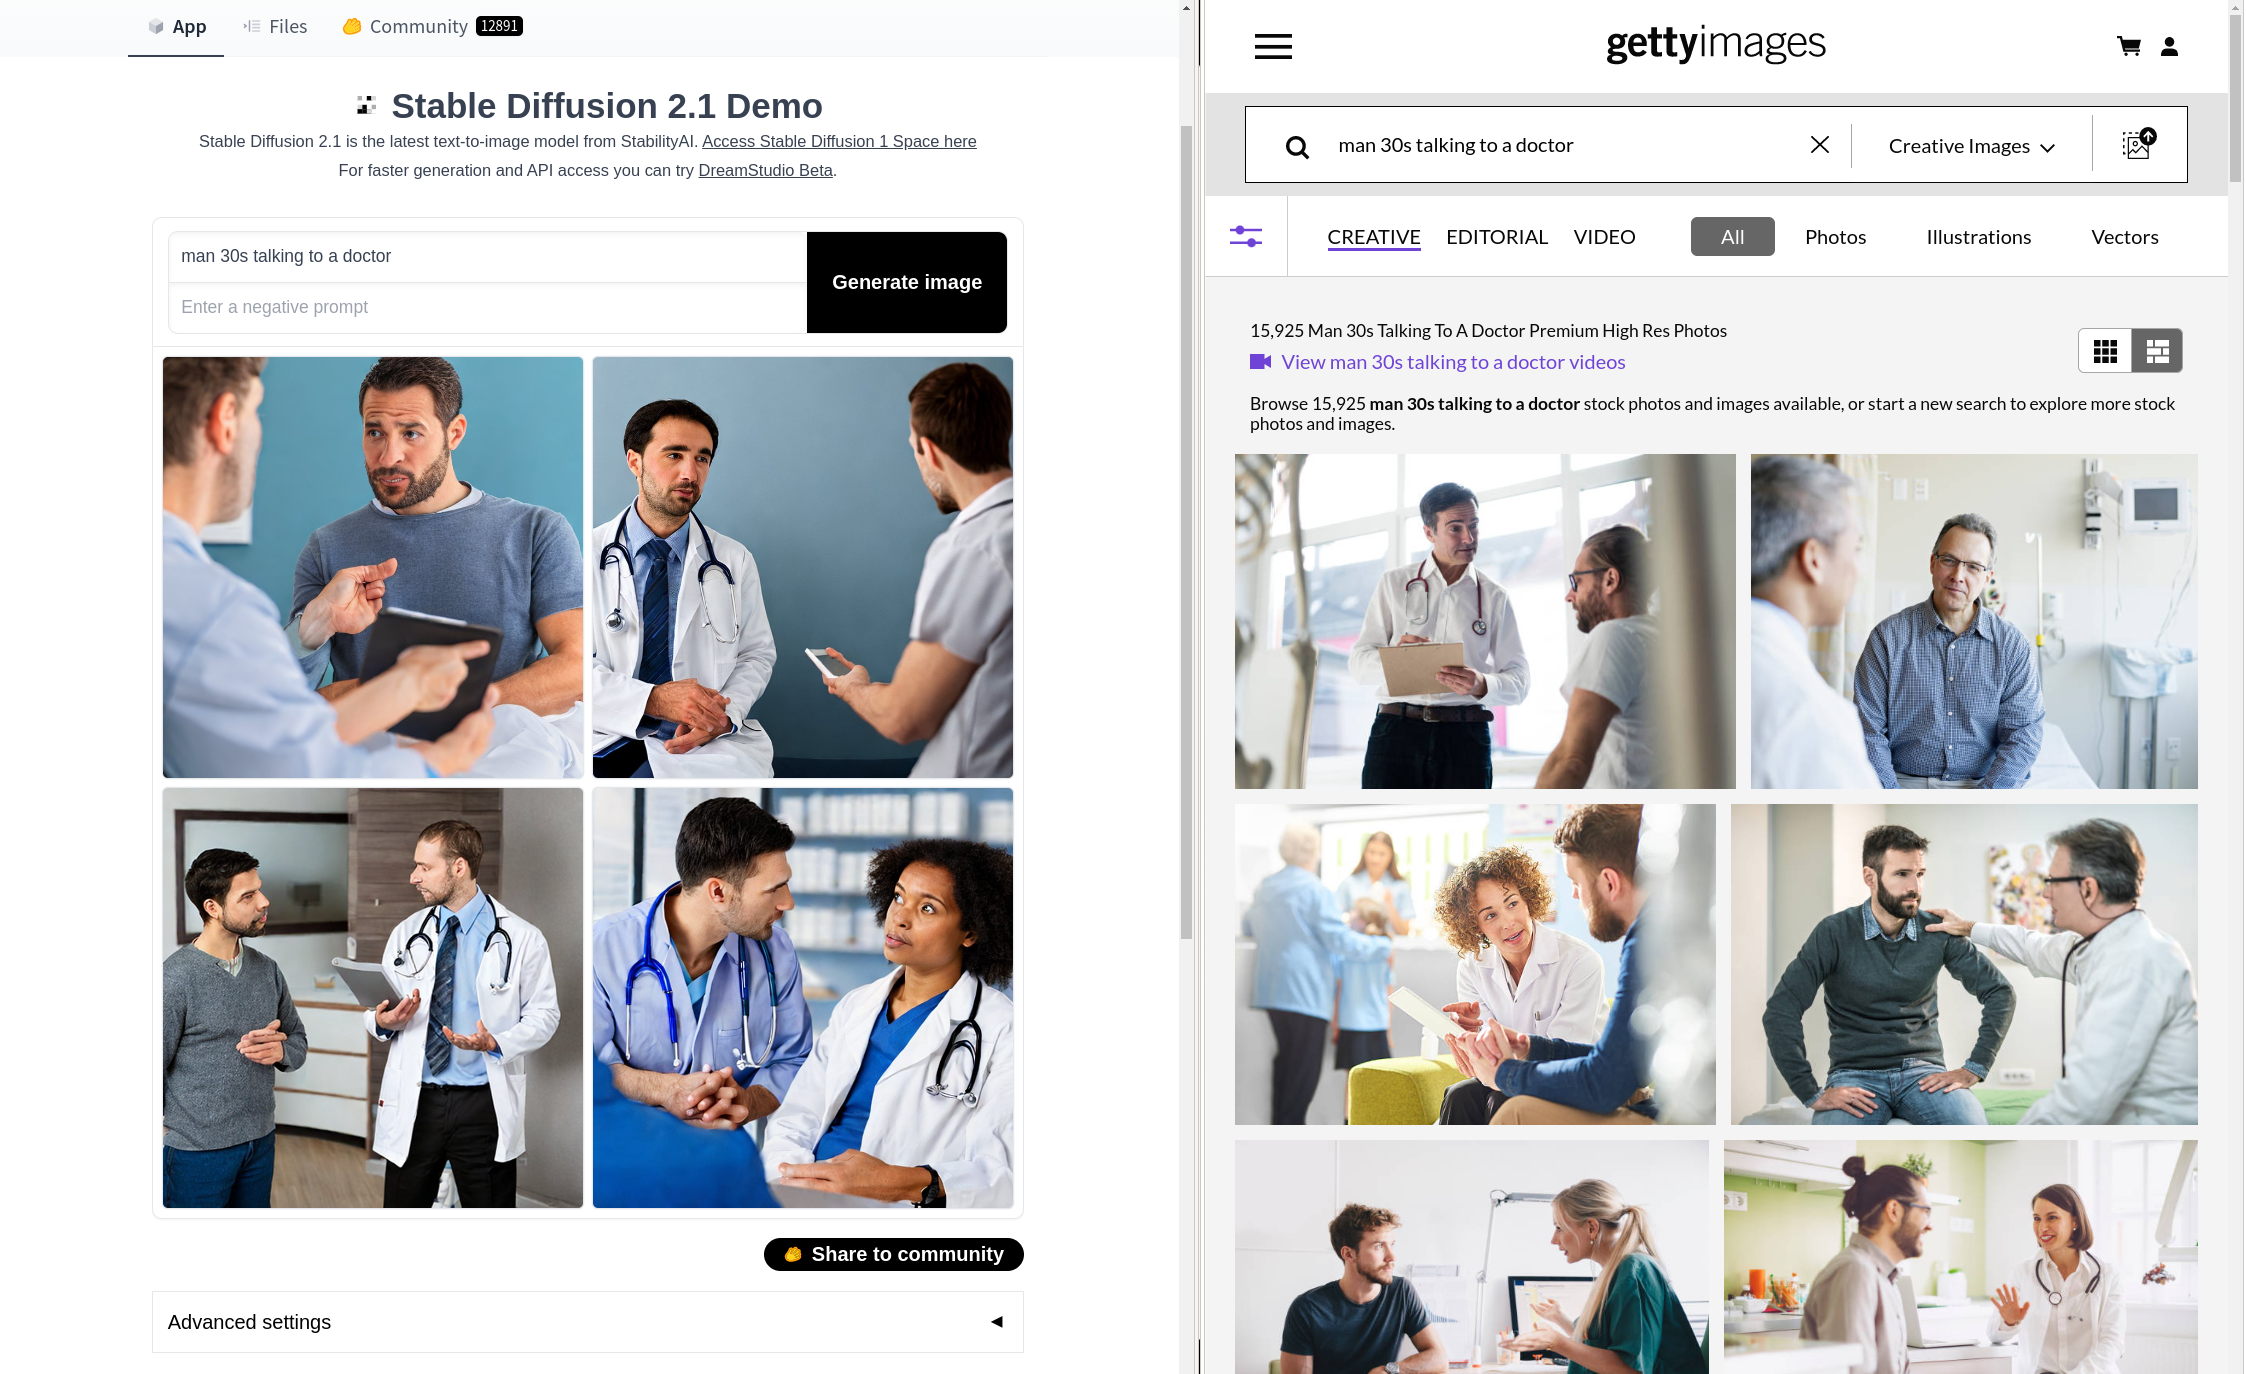
\includegraphics{getty}
        \caption{"man 30s talking to a doctor" Getty Images and Stable Diffusion comparison. Is Stable Diffusion creating something new here or spitting out it's training data? Is training a model like this fair use? I don't know, have fun lawyers! Note rights to each Getty photo runs around \$450, and Stable Diffusion is free to use, and they give users the rights to the model output. The Kraken has been released!}
        \labfig{getty}
\end{marginfigure}

These techniques can help to reduce the risk of having deep learning models reproduce the training data and cause intellectual property disputes, but there is no way to completely eliminate these risks, they are simply side-effects of the method of machine learning that we are doing nowadays. If you are an IP lawyer and need an expert witness, I'm your man \href{mailto:brad@bradflaugher.com}{brad@bradflaugher.com}.

\section{Working Together is Best}

It turns out sometimes the best combination is a reasonably smart (but not too cocky) human that gets to get recommendations from a few deep learning models. \sidenote{Funnily enough at Wharton I recently took \href{https://executiveeducation.wharton.upenn.edu/for-individuals/all-programs/effective-decision-making-thinking-critically-and-rationally/}{a class} where Dr. Cade Massey said basically "If you want to bring people along and get them to use your model, let them play with the output a bit, allowing for even the slightest bit (2\%) adjustment in the outputs will get users to adopt your model much faster." Thanks Cade!}

Garry Kasparov, the legendary chess player we heard about in chapter 1, witnessed a tournament where humans and AI could compete together. The tournament was designed to showcase the strengths of both humans and AI, and how they could work together to achieve incredible results here is what Garry says about the tournament:

\textit{"Once again, the chess world offers a useful test case for how this collaboration can play out. In 2005 the online chess playing site Playchess.com hosted what it called a "freestyle" chess tournament in which anyone could compete in teams with other players or computers. What made this competition interesting is that several groups of grandmasters working with computers also participated in this tournament. Predictably, most people expected that one of these grandmasters in combination with a supercomputer would dominate this competition ; but that's not what happened. The tournament was won by a pair of amateur American chess players using three computers. It was their ability to coordinate and coach effectively their computers that defeated the combination of a smart grandmaster and a PC with great computational power."}\sidecite{kasparov2005}

The tournament was a huge success, and showed that when humans and AI work together, they can achieve amazing things. The tournament participants learned that AI is not just a tool, but a valuable partner, and that by combining their strengths, they could achieve results that neither could have accomplished on their own. The tournament inspired many people to explore the potential of human-AI collaboration, and showed that by embracing technology, we can create a brighter future for all.

AI is an amazing partner, but we need to think for ourselves too. We can't blindly trust AI, but we can use it to inspire and challenge us.\sidecite{mansharamani2020}

\section{Key Takeaways}

\begin{itemize}
    \item \textbf{When you are using deep learning models, you are almost always engaging in some kind of transfer learning.} You are assuming the past will be like the future, or that training set reflects reality, which isn't always the case. \sidenote{It's as simple as the common financial disclaimer \textit{Past performance is no guarantee of future results.} Even though it is everywhere, the general public and even big swingers in finance don't seem to get this one. In AI there is an additional disclaimer, \textit{Training data may not reflect the the "real world".}}
    \item \textbf{Models can puke out seemingly creative things, but they are still a product of their training data.} deep learning models are deterministic systems, they slap together data based on rules they guessed from their training data. This process can still be very useful, but deep learning models are not sentient creative creatures from science fiction.
    \item \textbf{Even if you think you "own the rights" to the output of a model, models can sometimes puke out their training data} modelers try their best to prevent this but models can spit out their training data, which may cause headaches for everyone except the intellectual property lawyers. 
    \item \textbf{Users should consider the quality and appropriateness of the data the model they are using is trained on before deciding to use a model.} Remember, machine learning engineers spend most of their time cleaning up and gathering data, if you ask questions about how and when the data was collected and cleaned up you can get ahead of potential problems of concept drift and blind transfer learning (engaging in transfer learning without your consent).
    \item \textbf{Work with the technology} don't make your model do everything, sometimes it'll come up with stupid answers. Also don't assume you are always right, try and remember the story of the freestyle chess tournament and the grandmasters who got beat by the ameteurs getting reasonable advice from a few chess engines. Working with your model, as if it were a coworker that you don't fully trust, but still think is smart is probably the best way to use deep learning models.
\end{itemize}

 
%\setchapterpreamble[u]{\margintoc}
\chapter{Creativity and Decision Making with Deep Learning Models}
\labch{decisions}

\textit{"AI Policy}

\textit{I expect you to use AI (ChatGPT and image generation tools, at a minimum), in this class. In fact, some assignments will require it. Learning to use AI is an emerging skill, and I provide tutorials in Canvas about how to use them. I am happy to meet and help with these tools during office hours or after class}

\textit{Beware of the limits of ChatGPT:}

\begin{itemize}
	\item\textit{If you provide minimum effort prompts, you will get low quality results. You will need to refine you prompts to get good outcomes. This will take work.}
	\item\textit{Don't trust anything it says. If it gives you a number or a fact, assume it is wrong unless you either know the answer or can check in with another source. You will be responsible for any errors or omissions provided by the tool. It works best for topics you understand.}
	\item\textit{AI is a tool, but one that you need to acknowledge using. Please include a paragraph at the end of any assignment that uses AI explaining what you used the AI for and what prompts you used to get the results. Failure to do so is in violation of academic honesty policies}
	\item\textit{Be thoughtful about when this tool is useful. Don't use it if it isn't appropriate for the case or circumstance."}
\end{itemize}

\textit{Dr. Ethan Mollick, 2023 - Syllabus for class at The Wharton School at the University of Pennsylvania}


\section{Theories of Creativity}

Machine learning models use data (from the past) to discover rules and make classifications. Because of the way they are constructed these classifications, suggestions, artworks are by definition derivative or "having parts that originate from another source". I won't get into a philosophical discussion on what the nature of creativity is, but it's worth considering how using deep learning models biases us towards the past, but also could give us insights from other domains. 

\begin{marginfigure}[-5.5cm]
        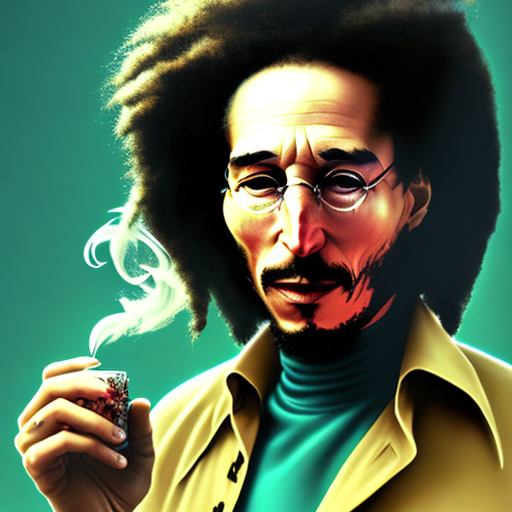
\includegraphics{jobsweed}
        \caption{"mdjrny-v4 Steve Jobs Smoking weed with Bob Marley 8k" made with Mann-E. It's 100\% derivative, but it's art too (I guess).}
        \labfig{jobsweed}
\end{marginfigure}

It can be argued that creativity is simply the combination of existing works. This is because many new ideas and innovations are often inspired by and built upon existing concepts. For example, a new form of music may be created by combining elements from different genres. Similarly, a new technology may be created by combining and improving upon existing technologies.

It can also be argued that creativity involves much more than just combining existing works. Creativity is not just about recombining existing ideas, but also about coming up with completely new and original concepts. This requires a unique perspective and a deep understanding of the subject matter, as well as the ability to think outside the box.  

Deeep learning models of speech, when heavily used, may slow down the evolution of language. AI art models may slow down "progress" in art, whatever that means. Deep learning models of disease trained on data from 1980 may be irrelevant to today's diseases. That said these same models may give us interesting insights in new domains, models trained on beautiful paintings may be put to use in a new domain (like designing beautiful interiors) and that model could give new insight to interior designers, models of the interaction of ants could be put to use in designing cities and so on and so forth. AI cuts many ways, it makes us faster but makes us more reliant on the past, models can be used across domains but should be used intentionally and transparently when possible. Each use opens up a new world of possibilities for users, and sometimes a new headache for intellectual property lawyers. We'll discuss all of these topics in this chapter.

\begin{marginfigure}[-5.5cm]
        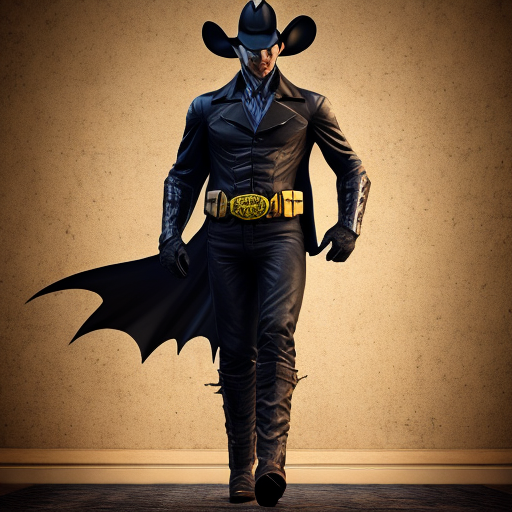
\includegraphics{batman}
        \caption{"Batman dressed as a cowboy" made with Mann-E. It's 100\% derivative as well, but better than any Google image searches I did. It looks amazing! I also might get sued if I use it even though the creators of Mann-E tell me I have the rights to it.}
        \labfig{batman}
\end{marginfigure}

\section{Creative Uses of Power Tools}

Power tools, even simple ones like a drill are complex machines that take human input and transform it using static rules. The pressure the user of a drill puts on the bit and the speed at which they pull the trigger all deterministically affect the output. Just because a tool is a deterministic machine doesn't mean it is unable to produce creative works.

What is happening as we use generative tools like ChatGPT or image-to-text models is that the "creative act" has been relocated. The creative act is now the prompt you give the tool, the users input. And someone can still be good at using AI, just like someone can be good at using any piece of software.

Modern AI is a complex system of algorithms, data, and analytics that can be used to solve complex problems. AI systems can learn from data, identify patterns, and make predictions about the future. AI systems are typically used to automate and assist human decision making. AI systems are programmed with specific objectives and goals, and the user input decides the output. For example, an AI system could be programmed to solve a mathematical problem and the user input would determine the parameters of the problem and the output would be the solution.

A power drill is also a complex deterministic system. The user input is limited to the type of drill bit, the speed of the drill, and the direction of the drill. The output is determined by these inputs, as the drill will only drill in the direction and speed determined by the user. The user also has to choose the correct drill bit to ensure the drill can do the job correctly and safely.

\begin{marginfigure}[-5.5cm]
        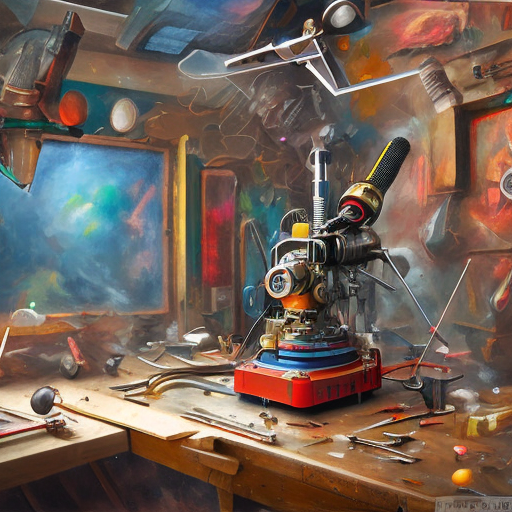
\includegraphics{drillart}
        \caption{"mdjrny-v4 a mikita drill being used in an artist's studio to make a colorful artwork 8k" made with Mann-E}
        \labfig{drillart}
\end{marginfigure}

Both modern deep learning models and a power drill are complex but ultimately deterministic systems. The user input, however limited it may be, ultimately controls the output of the system. Both systems require a user to understand how to use them and to make the correct input to get the desired output.

\section{Garbage In, Garbage Out}
\labsec{creative}

The "Power Tool" of AI is a deterministic, static and unchanging system and the rules of that system are determined by the data that the model is shown. If a model is trained on bad data, it will produce poor results. End of book...

... maybe not. It's worth thinking about this for a moment. It is often said that modern AI can "generalize and make informed inferences given new data". If deep learning models are really just a big regression, these models will always come up with an answer, but if the world changes, these models will still be projecting complicated averages of their past data into the future. 

So, let's separate AI's decision making into two extremes; \textit{Creative Decision Making} and \textit{Critical Decision Making}. The stakes are very low in a world of \textit{Creative Decision Making} and who cares if the AI is all a regression, and it just mushes together the limited data that it's seen. In a creative context you can also ask an AI interesting questions, so long as you don't solely rely on it's output without checking the facts first\sidenote{See the syllabus note from Dr. Mollick at the beginning of this chapter.}. Even if "Garbage In, Garbage Out" holds, garbage can still be helpful for a creative process. 

Note that this book is called "Full-Self Driving, Skynet..", a self-driving car and a nuclear-bomb-equipped all-seeing AI are clearly not engaging in any \textit{Creative Decision Making}. 

\section{Garbage In, New Perspective Out?}

For creative tasks, it generally doesn't matter that a deep learning model is unscientific or trained on a lopsided dataset. An informed user of AI knows this and can account for that in their decision making, especially when engaging in creative decision making. The situation becomes problematic once we allow deep learning models to engage in critical decision making by themselves. 

\begin{marginfigure}[-5.5cm]
        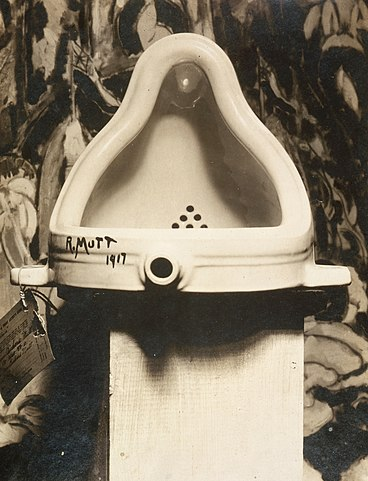
\includegraphics{duchamp}
        \caption{Marcel Duchamp's "Fountain". A urinal that blew peoples minds \url{https://www.tate.org.uk/art/artworks/duchamp-fountain-t07573}.}
        \labfig{duchamp}
\end{marginfigure}

Generative models will come up with amazing (but derivative) works of art, But, they will never "change the game". A model of sculpture trained on past sculptures in 1917 will never come up with Marcel Duchamp's "Fountain". There is a term that machine learning engineers use for this, when the rules of the game are changed, it's called "Concept Drift".

\section{Concept Drift and the End of Usefulness}
\labsec{drift}

Concept drift refers to the phenomenon where the distribution of data changes over time, causing the performance of deep learning models built on historical data to degrade. The model becomes less useful because it is trained to make predictions based on the relationship between the inputs and outputs in the data it was trained on, and if this relationship changes, the model may start making incorrect predictions. This is particularly problematic in real-world applications, where the data is constantly evolving and the relationship between inputs and outputs is subject to change. To mitigate the effects of concept drift, it is often necessary to continually retrain deep learning models on updated data.

The frequency with which a deep learning model needs to be retrained to mitigate the effects of concept drift depends on several factors, including the rate at which the data distribution changes, the size and complexity of the model, and the availability of computational resources.

For some applications with relatively stable data distributions, retraining the model once every few months or even once per year may be sufficient. However, in other applications where the data is changing rapidly, it may be necessary to retrain the model more frequently, such as once per week or even once per day.

\begin{marginfigure}[-5.5cm]
        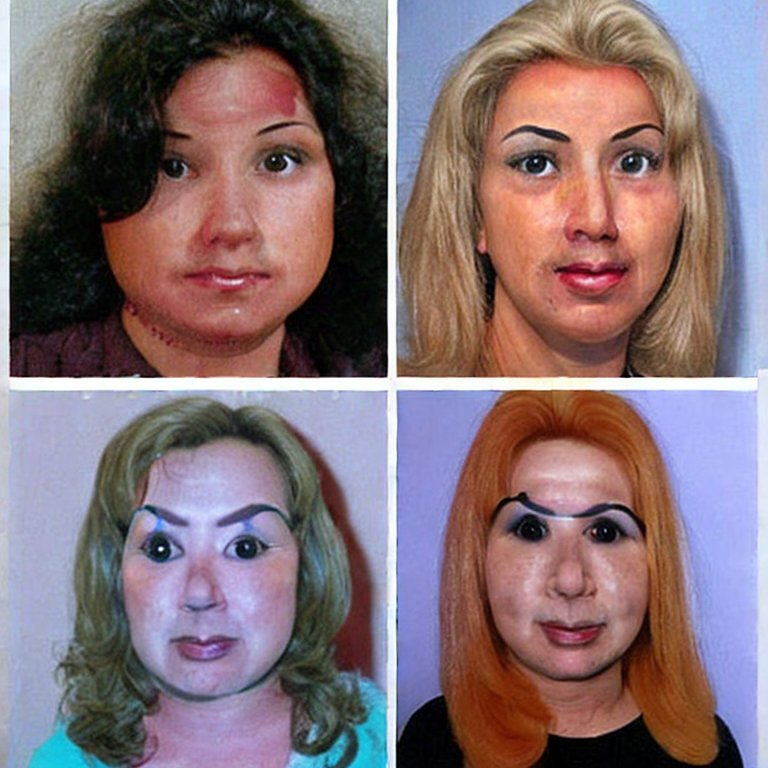
\includegraphics{plastic}
        \caption{"Plastic surgery gone wrong" made with Stable Diffusion. Imagine a model that classifies images as "human face" or "not human face", and imagine that model was trained on images of human faces before 1900, maybe you would not be surprised if you gave it a picture of a human face that had a lot of cosmetic surgery done to it, and that model might say "this is not a human face", the idea of what a human face is has changed over time this is called "concept drift".}
        \labfig{plastic}
\end{marginfigure}

Ultimately, the frequency of retraining will depend on the specific requirements of the application, and the trade-off between the cost of retraining and the potential cost of incorrect predictions. In general, it's recommended to monitor the performance of the model over time and to retrain it as needed to ensure that it remains accurate and relevant.

If a deployed deep learning model is not monitored, there are several risks that can emerge:

\begin{itemize}
\item Accuracy degradation: As the data distribution changes over time, the model may become less accurate, leading to incorrect predictions. This can result in financial losses, reduced customer satisfaction, or even harm to individuals.
\item Bias amplification: deep learning models can be biased, and if this bias is not monitored and addressed, it can be amplified over time as the model continues to make incorrect predictions. This can result in discriminatory outcomes, such as unequal treatment of individuals based on protected characteristics such as race, gender, or age.
\item Legal liability: In some cases, incorrect predictions made by deep learning models can result in legal liability, particularly if the model is being used to make decisions that have significant consequences, such as in the criminal justice system or in medical diagnosis.
\item Reputational damage: If a deep learning model is making incorrect predictions, it can damage the reputation of the organization deploying the model, potentially leading to a loss of customers or investors.
\end{itemize}


It is important to monitor deep learning models once they are deployed, and to take action to address any issues that arise, such as retraining the model or adjusting its parameters, in order to mitigate these risks and ensure that the model continues to perform well over time.

\section{The Impossibility of Fairness}

Achieving fairness in deep learning models can be challenging, and to some extent it may be impossible to completely eliminate all forms of bias. This is because deep learning models are trained on historical data, which may contain biases and disparities that are perpetuated in the model's predictions. One can attempt to "fix the training set" but in practice models will continue to bias their prediction to past data, or their creators careful curation of the past.\sidecite{Christian2020} 

However, it is possible to reduce the impact of bias in deep learning models through careful design and monitoring of the model's performance. This may include techniques such as fairness constraints, algorithmic transparency, and regular auditing of the model's predictions to identify and address any issues of bias.

It's important to note that fairness is a complex and multi-faceted concept, and different definitions of fairness may be appropriate for different applications. For example, some definitions of fairness may prioritize equal treatment of all individuals, while others may prioritize proportional representation or equal opportunities.

Ultimately, the extent to which fairness is achievable in deep learning models will depend on the specific requirements of the application and the level of effort that is put into designing and monitoring the model to ensure that it is making fair and unbiased predictions.

\section{Transfer Learning Everywhere}

Transfer learning is a machine learning technique that involves transferring knowledge from one model trained on a task to another model trained on a related task. The idea behind transfer learning is that a model that has been trained on one task can be fine-tuned for another task, reducing the amount of labeled data required to train the new model.

For example, imagine that you have a deep learning model that has been trained to recognize objects in natural images (cats, dogs, balls, cars). You can use the knowledge learned by this model as a starting point to train a new model that recognizes objects in medical images, such as X-rays or MRI scans. The new model can start with the weights of the pre-trained model and fine-tune them on the new task, using a much smaller amount of labeled data than would be required to train the model from scratch.

Transfer learning can be useful in many different applications, particularly when labeled data is scarce or expensive to obtain. By leveraging knowledge from a pre-trained model, transfer learning can help to improve the performance of new models, reduce the amount of data required for training, and accelerate the development of new machine learning applications.

I asked ChatGPT to "tell me a story of transfer learning going horribly wrong in the context of online dating, with a model trained in the Middle East being deployed by an American dating app." and here's what it said:

\textit{"Once upon a time, an American online dating company decided to use transfer learning to improve their matchmaking algorithms. They trained a state-of-the-art machine learning model on a large dataset of profiles and dating preferences from the Middle East. The model was able to suggest matches with remarkable accuracy and the company was confident that it would perform just as well in the American market.}

\textit{However, things went terribly wrong when they deployed the model on their American dating app. The model was not properly trained to consider the cultural and social differences between the Middle East and America. As a result, it suggested matches that were inappropriate and offensive, causing widespread backlash and criticism from users.}

\textit{For example, the model suggested matches between people of different religious backgrounds, which was not acceptable to many users. It also suggested matches between people with significant age gaps, which was not socially acceptable in the American market.}

\textit{The company was forced to remove the model and start from scratch, causing significant harm to their reputation and financial losses. They learned the hard way that transfer learning can only be effective if the model is properly trained on relevant and culturally appropriate data.}

\textit{This story serves as a cautionary tale about the importance of considering cultural differences and ethical implications when deploying machine learning models in different regions and markets."}

Not bad I think... picking good training data and doing good "data janitoring" is the main job of a machine learning engineer\sidenote{The better your machine learning engineer understands your business problem, the better job they'll do at creating the dataset.}.

If the past is not like the future, you are also doing transfer learning. Most models steal data from other sources so are doing transfer learning too. This is fine, but do we know that we are doing this? A model that is deployed in a domain experiencing concept drift and continues to make predictions without being retrained can be considered to be doing a harmful form of transfer learning. This is because the model has been trained on a different distribution of data (the past), and is being applied to a new domain with a different distribution (the present and future).

In traditional transfer learning, the goal is to transfer knowledge from one domain to another related domain, where the data distributions are similar enough to enable the model to make accurate predictions. However, in the case of concept drift, the data distributions are changing over time, and the model is becoming less accurate as a result. \sidenote{Think about your life and if you "transferred" your model of thinking from when you were 12 years old, to "today" when you are 35 years old, that is a bad model to be operating on! That model needs to be updated. We'll explore many examples of where this is and is not a problem in the next chapter."}

By continuing to make predictions without being retrained, the model is essentially "transferring" its knowledge from a historical data distribution to a new, changed data distribution, which may not be a valid assumption. This can result in incorrect predictions and other negative outcomes, such as harm to individuals or organizations.

\section{Industrial-Scale Plagiarism}
\labsec{plag}

Aside from regurgitating the past and predictions from other domains, deep learning models can also enable plagiarism on an industrial scale. Early text generation models could be made to write entire sections of \textit{Harry Potter} when fed the opening lines of a chapter. Even as models grow large and more sophisticated, users, researchers and lawyers are still able to "extract the training data"  from large models\sidecite{Carlini2023}, causing headaches for their creators and adding to the work of intellectual property lawyers. 

To avoid this creators of deep learning models have the following tools at their disposal:


\begin{itemize}
\item Best practices in  machine learning: data preprocessing, augmentation, reuglarization, model architecture choices, early stopping and validation are all things that we are taught to do to prevent overfitting.
\item Contractual agreements: Microsoft (owner of github and cocreator of the \href{https://github.com/features/copilot}{Github Copilot} code generation model) has a special contract for anyone submitting code to github that essentially says that "we are allowed to use this code to train our models, and if our models regenerate your copyrighted code, you can kick rocks."
\item Release the Kraken: StabilityAI's Stable Diffusion model was released as open source software, they still managed to get sued \cite{getty}, but they basically said, "this model was trained on all copyrighted and copylefted images on the web, sometimes it'll generate stuff that violates copyright law, but we are in Germany and will give this thing away for free to the public, and see how Getty Images, photographers and graphic designers of the world handle it... good luck!". 
\end{itemize}


\begin{marginfigure}[-5.5cm]
        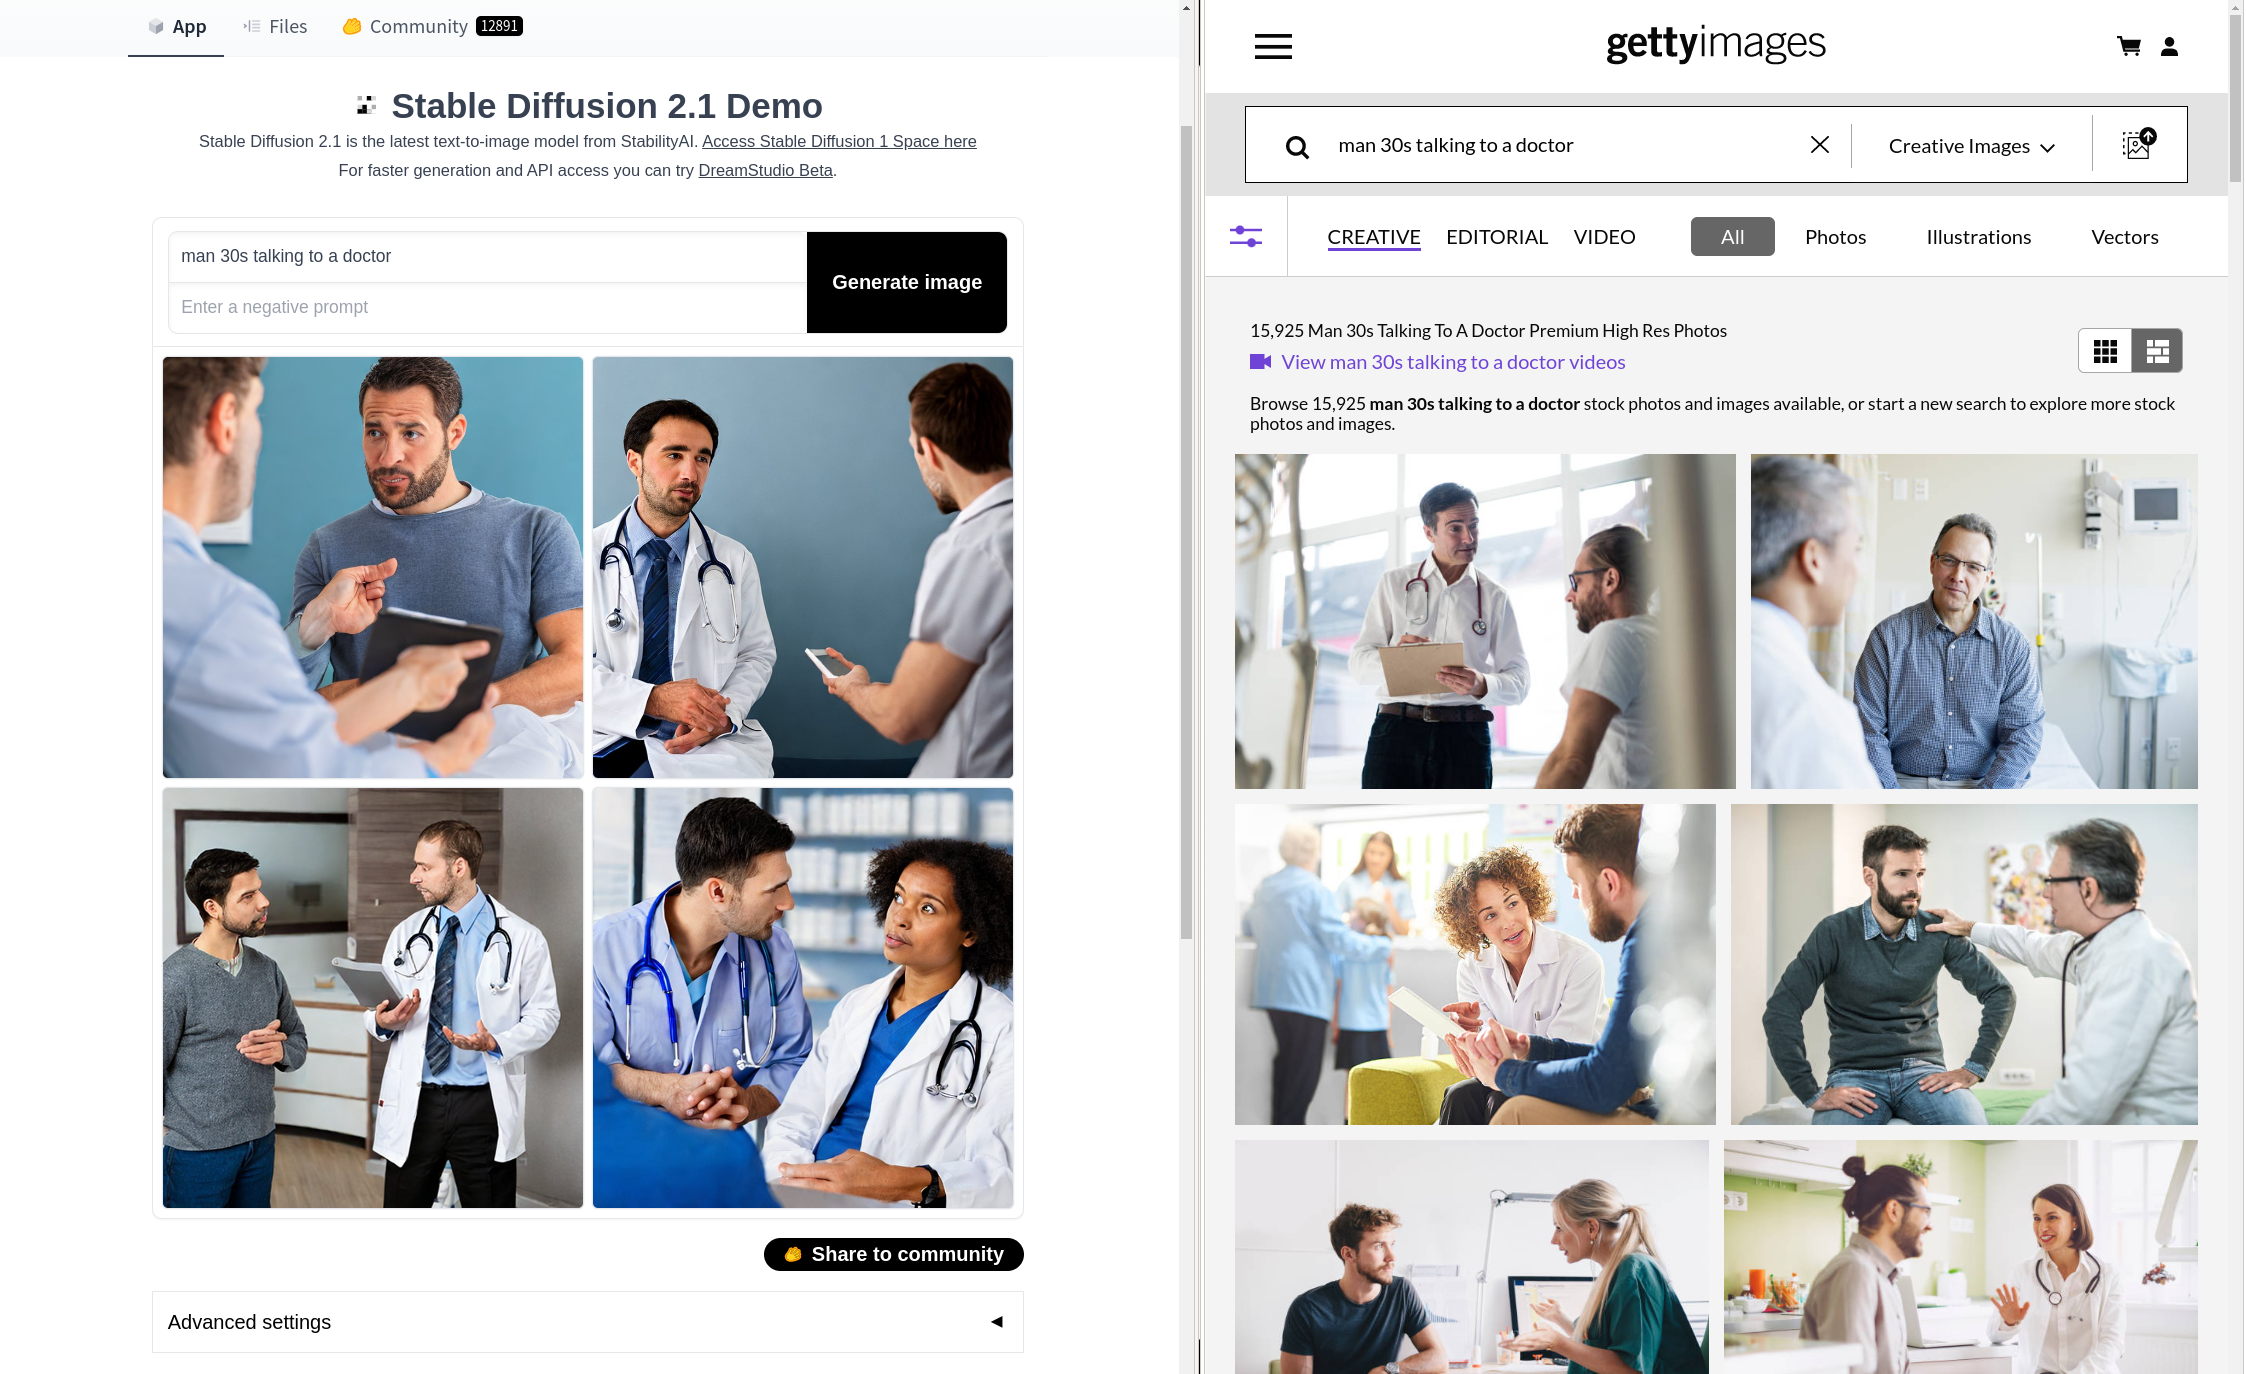
\includegraphics{getty}
        \caption{"man 30s talking to a doctor" Getty Images and Stable Diffusion comparison. Is Stable Diffusion creating something new here or spitting out it's training data? Is training a model like this fair use? I don't know, have fun lawyers! Note rights to each Getty photo runs around \$450, and Stable Diffusion is free to use, and they give users the rights to the model output. The Kraken has been released!}
        \labfig{getty}
\end{marginfigure}

These techniques can help to reduce the risk of having deep learning models reproduce the training data and cause intellectual property disputes, but there is no way to completely eliminate these risks, they are simply side-effects of the method of machine learning that we are doing nowadays. If you are an IP lawyer and need an expert witness, I'm your man \href{mailto:brad@bradflaugher.com}{brad@bradflaugher.com}.

\section{Working Together is Best}

It turns out sometimes the best combination is a reasonably smart (but not too cocky) human that gets to get recommendations from a few deep learning models. \sidenote{Funnily enough at Wharton I recently took \href{https://executiveeducation.wharton.upenn.edu/for-individuals/all-programs/effective-decision-making-thinking-critically-and-rationally/}{a class} where Dr. Cade Massey said basically "If you want to bring people along and get them to use your model, let them play with the output a bit, allowing for even the slightest bit (2\%) adjustment in the outputs will get users to adopt your model much faster." Thanks Cade!}

Garry Kasparov, the legendary chess player we heard about in chapter 1, witnessed a tournament where humans and AI could compete together. The tournament was designed to showcase the strengths of both humans and AI, and how they could work together to achieve incredible results here is what Garry says about the tournament:

\textit{"Once again, the chess world offers a useful test case for how this collaboration can play out. In 2005 the online chess playing site Playchess.com hosted what it called a "freestyle" chess tournament in which anyone could compete in teams with other players or computers. What made this competition interesting is that several groups of grandmasters working with computers also participated in this tournament. Predictably, most people expected that one of these grandmasters in combination with a supercomputer would dominate this competition ; but that's not what happened. The tournament was won by a pair of amateur American chess players using three computers. It was their ability to coordinate and coach effectively their computers that defeated the combination of a smart grandmaster and a PC with great computational power."}\sidecite{kasparov2005}

The tournament was a huge success, and showed that when humans and AI work together, they can achieve amazing things. The tournament participants learned that AI is not just a tool, but a valuable partner, and that by combining their strengths, they could achieve results that neither could have accomplished on their own. The tournament inspired many people to explore the potential of human-AI collaboration, and showed that by embracing technology, we can create a brighter future for all.

AI is an amazing partner, but we need to think for ourselves too. We can't blindly trust AI, but we can use it to inspire and challenge us.\sidecite{mansharamani2020}

\section{Key Takeaways}

\begin{itemize}
    \item \textbf{When you are using deep learning models, you are almost always engaging in some kind of transfer learning.} You are assuming the past will be like the future, or that training set reflects reality, which isn't always the case. \sidenote{It's as simple as the common financial disclaimer \textit{Past performance is no guarantee of future results.} Even though it is everywhere, the general public and even big swingers in finance don't seem to get this one. In AI there is an additional disclaimer, \textit{Training data may not reflect the the "real world".}}
    \item \textbf{Models can puke out seemingly creative things, but they are still a product of their training data.} deep learning models are deterministic systems, they slap together data based on rules they guessed from their training data. This process can still be very useful, but deep learning models are not sentient creative creatures from science fiction.
    \item \textbf{Even if you think you "own the rights" to the output of a model, models can sometimes puke out their training data} modelers try their best to prevent this but models can spit out their training data, which may cause headaches for everyone except the intellectual property lawyers. 
    \item \textbf{Users should consider the quality and appropriateness of the data the model they are using is trained on before deciding to use a model.} Remember, machine learning engineers spend most of their time cleaning up and gathering data, if you ask questions about how and when the data was collected and cleaned up you can get ahead of potential problems of concept drift and blind transfer learning (engaging in transfer learning without your consent).
    \item \textbf{Work with the technology} don't make your model do everything, sometimes it'll come up with stupid answers. Also don't assume you are always right, try and remember the story of the freestyle chess tournament and the grandmasters who got beat by the ameteurs getting reasonable advice from a few chess engines. Working with your model, as if it were a coworker that you don't fully trust, but still think is smart is probably the best way to use deep learning models.
\end{itemize}

 
%\setchapterpreamble[u]{\margintoc}
\chapter{Self-Driving With Statistics}
\labch{intro}

\begin{itemize}
    \item\textit{First Law: A robot may not injure a human being or, through inaction, allow a human being to come to harm.}
    \item\textit{Second Law: A robot must obey the orders given it by human beings except where such orders would conflict with the First Law.}
    \item\textit{Third Law: A robot must protect its own existence as long as such protection does not conflict with the First or Second Law.}
\end{itemize} 
\textit{Asimov's Three Laws of Robotics}

\section{Self-Driving Horses}

\section{Semiautonomy is Stupid}

Talk about the levels 0-4, deep learning is a subsystem of these levels.

Semiautonomy is dumb because it feels autonomous, but the user is expected to take over at any time. This is the worst of both worlds. \cite{torchinsky_boeckmann_2019}

and this article \href{https://www.theautopian.com/newly-released-video-of-thanksgiving-day-tesla-full-self-driving-crash-demonstrates-the-fundamental-problem-of-semi-automated-driving-systems/}{Tesla Crash Illustrates Problem With Semi-Automated Driving} and \href{https://news.ycombinator.com/item?id=34347778}{comments}

\section{Trolley Problems}

\section{Concept Drift (Reprise)}

\section{Multicolinearity (Reprise)}

\sidenote{You can't get your self-driving car dirty either, it'll mess up those sensors.}

\section{Explaining The Unexplainable in Court}

\textit{"Limitations and Pitfalls of Explainable and Interpretable Methods}

\textit{Before diving into the exact methods for interpreting and explaining models, let's take a look at some of the pitfalls of these methods.}

\textit{First off, if you need to make high-stakes decisions, make sure to use inherently interpretable models. These are models such as decision trees that are more readily converted to output explanations.}

\textit{Before choosing a method, you need to be absolutely clear about what you want out of it. Are you trying to understand the nature of the data procurement process? How a decision was made? How the model works on a fundamental level? Some tools might be appropriate for some of these goals but not others.}

\textit{If your goal is to make sense of the data generation process, this is only possible if you know that your model already generalizes well to unseen data.}

\textit{Decision interpretability can be misleading. It highlights things like correlations, but doesn’t go into the level of causal detail that causal inference does. Remember that correlation does not (always) imply causation.}

\textit{WARNING}
\textit{Spurious correlations can result in inaccurate interpretations even with advanced interpretability methods like saliency methods and attention-based methods.}

\textit{Tools such as feature importance usually estimate mean values, but one should beware the error bars on those means and take stock of the confidence intervals.}

\textit{A lot of machine learning involves working with extremely high-dimensional spaces. There's no way around it: high-dimensional data and feature spaces are hard to make sense of without grouping the data or features together first.}

\textit{Even if you do find important features in those matrices, remember that this does not imply causality (we've said this before and we'll say it again)."} \cite{}

\section{A Train is a Self-Driving Car, Right?}

Discuss how the problem space has changed in warehousing, we don't actually have self-driving forklifts, we have moving shelves.

Maybe talk about elon musk and manufacturing.
 
%\setchapterpreamble[u]{\margintoc}
\chapter{Self-Driving with Statistics}
\labch{driving}

\textit{"We think of automation as a machine doing a task that a human used to do... you might think that means a human does nothing. But in fact there's abundant literature that shows the human is not incurring no workload, the human is now doing a different task and that task tends to be monitoring, a vigilance task, looking for rare events...that is a task that humans are not well-equipped to do." - Dr. Michael Nees, 2021} \cite{nees2021}


\section{The Dangers of Semi-Autonomy}

Two hundred years ago, horses were the most sophisticated mode of transportation. They possessed an innate ability to navigate terrain and avoid obstacles, even without a human rider at the reins. People often took comfort in the horse's natural instincts, which allowed for moments of respite during long journeys. Fast forward to today, where we have vehicles that claim to possess similar levels of autonomy, but with significantly more horsepower (pun intended).

One might be tempted to compare these self-driving cars to our trusty equine friends, imagining a world where vehicles, like horses, can be left to their own devices. Alas, this comparison is a misleading one, as it creates the illusion that our self-driving cars are more capable than they currently are.

The National Highway Traffic Safety Administration (NHTSA) has devised a six-level classification system to describe vehicle autonomy, ranging from Level 0 (no automation) to Level 5 (full automation). Most commercially available vehicles today hover between Levels 2 and 3, providing advanced driver assistance but requiring constant human oversight. This semi-autonomous state can lull drivers into a false sense of security, prompting them to disengage from the driving task in a manner that might have been acceptable during the days of horse-drawn carriages but is decidedly dangerous in the modern era.

\begin{pdf}
\begin{marginfigure}[-5.5cm]
        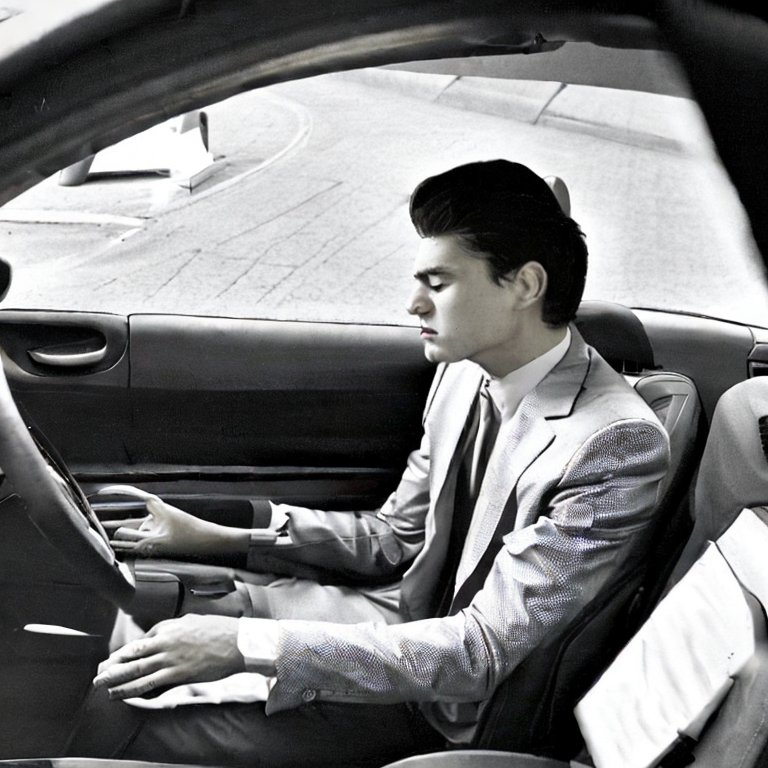
\includegraphics{asleep}
        \caption{"style a person in a business suit asleep at the wheel of a car AP" made with Stable Diffusion 2.1}
        \labfig{asleep}
\end{marginfigure}
\end{pdf}

In his book "Robot Take the Wheel," author Jason Torchinsky offers a compelling argument against semi-autonomy, dubbing it "stupid" in a section bearing the same name. Torchinsky highlights the impracticality of expecting a driver who has relinquished control to a semi-autonomous system to suddenly take over in a moment of crisis. Manufacturer warnings, while intended to encourage drivers to stay attentive, often go unheeded, creating a precarious situation where those behind the wheel are ill-prepared to intervene when the technology falters.\sidecite{torchinskyboeckmann2019}

The world of transportation extends beyond the realm of four-wheeled automobiles. The skies above host a veritable ballet of commercial aircraft, which rely on sophisticated autopilot systems to ferry passengers and cargo across vast distances. These systems differ in important ways from automobile autopilot and have significantly different infrastructure (not to mention terrain, or lack thereof).In aviation, autopilots demand constant monitoring and communication between the pilot, the aircraft, and air traffic control. In many ways, the intricacies and collaboration required for safe air travel can serve as a model for understanding the complexities of developing and implementing truly autonomous ground vehicles.

\section{Comparing Autopilot Systems}

At a glance, the autopilot systems in airplanes and Teslas may seem to share common goals: both strive to provide increased safety, efficiency, and convenience. However, the similarities largely end there, as the underlying technologies and the environments in which they operate diverge significantly.

Commercial airplanes, for example, are equipped with highly sophisticated autopilot systems capable of managing tasks such as altitude, speed, and heading control. In contrast, Tesla's advanced driver-assistance system (ADAS), while advanced, is focused primarily on lane keeping, adaptive cruise control, and collision avoidance. Furthermore, the aviation industry has a long history of integrating automation with well-established regulations, procedures, and training, whereas the automotive industry is still in the early stages of defining standards and best practices for autonomous vehicles.

One critical aspect of aircraft autopilot systems is the need for seamless communication and coordination with external systems, such as air traffic control (ATC) and other aircraft. This level of coordination ensures that each plane maintains a safe distance from others, follows established routes, and adheres to ATC instructions.

On the other hand, vehicles like Teslas currently have limited means of communication with external systems, relying instead on onboard sensors and mapping data to navigate the environment. As autonomous vehicle technology advances, however, it is anticipated that vehicle-to-vehicle (V2V) and vehicle-to-infrastructure (V2I) communication will become increasingly important for coordinating traffic flow and maintaining safety.

\begin{pdf}
\begin{marginfigure}[-5.5cm]
        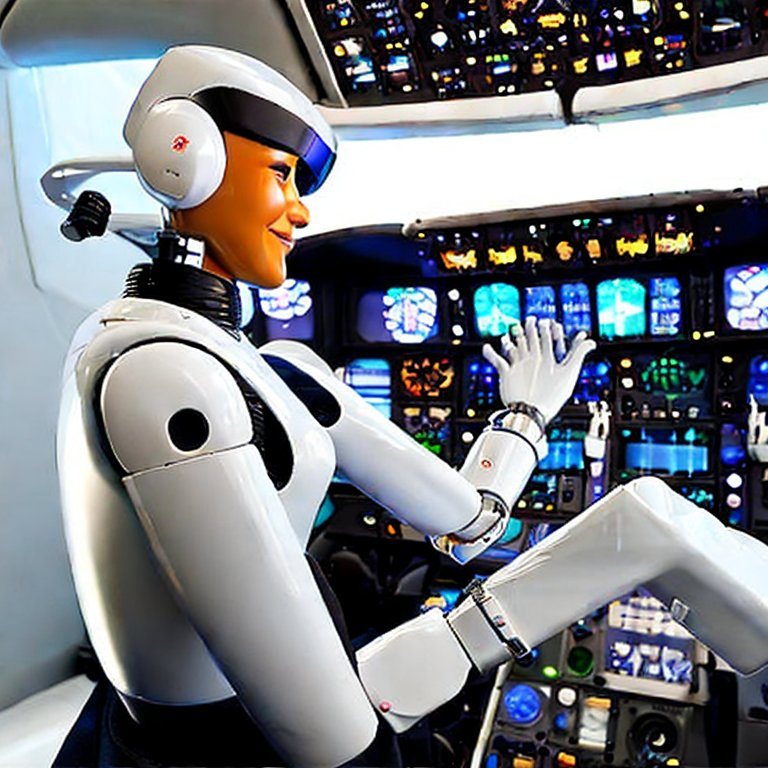
\includegraphics{pilot}
        \caption{"a robot pilot at the helm of a commercial airliner, being served by a human flight attendant" made with Stable Diffusion 2.1}
        \labfig{pilot}
\end{marginfigure}
\end{pdf}

Despite the advanced nature of aircraft autopilot systems, pilots are still required to maintain a constant vigil, monitoring the system and intervening when necessary. This level of human oversight is not only mandated by regulations but also reinforced through rigorous training and the understanding that even the most advanced systems can fail.

In contrast, drivers of vehicles equipped with ADAS, such as Teslas, often face the temptation to over-rely on the technology and disengage from the driving task, as discussed in the previous section. This discrepancy highlights the need for clear guidelines and education on the proper use of semi-autonomous systems in cars, to ensure that drivers remain vigilant and prepared to intervene when needed.

\section{Who Should The Car Kill?}

In this section, we delve into the ethical dilemmas that arise when designing autonomous vehicles. We will discuss the Trolley Problem and its application to autonomous decision-making, as well as the legal and moral considerations of outsourcing responsibility to machines.

The Trolley Problem, a classic thought experiment in ethics, poses a hypothetical scenario where an individual must choose between two undesirable outcomes, often involving the deaths of different groups of people. In the context of autonomous vehicles, the Trolley Problem raises the question of how a self-driving car should prioritize the safety of its occupants, pedestrians, and other road users in situations where an accident is unavoidable.

As developers of autonomous vehicles grapple with these ethical quandaries, they must decide what values and priorities to embed in their algorithms. Should a self-driving car prioritize minimizing overall harm, protecting its passengers, or adhering to specific legal and moral rules? The choices made in designing these systems will have profound implications for society, as they will determine how autonomous vehicles respond in life-or-death situations.

The advent of autonomous vehicles raises complex questions about responsibility and liability. If a self-driving car is involved in an accident, who should be held accountable – the vehicle's owner, the manufacturer, or the software developer? As we outsource decision-making to machines, we must grapple with the legal and moral implications of this shift.

One potential approach is to establish a new legal framework that recognizes the unique nature of autonomous vehicles, assigning responsibility based on factors such as the level of autonomy, the specific circumstances of an accident, and the degree of human oversight. This would likely involve a combination of civil and criminal liability, as well as new insurance models to address the changing landscape of risk.

\begin{pdf}
\begin{marginfigure}[-5.5cm]
        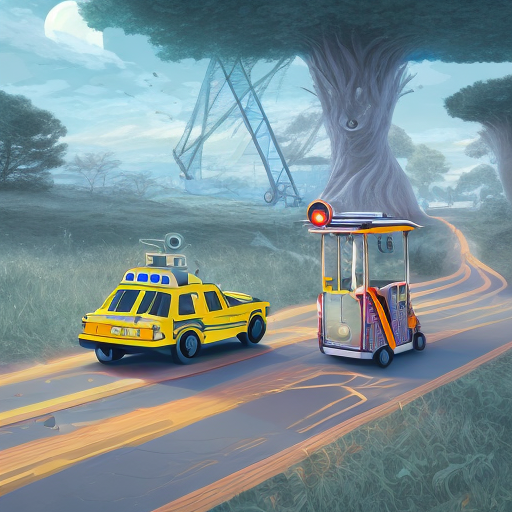
\includegraphics{trolley}
        \caption{"mdjrny-v4 A humorous, cartoonish illustration of an autonomous vehicle facing the classic trolley problem 8k" made with Stable Diffusion 2.1}
        \labfig{trolley}
\end{marginfigure}
\end{pdf}

From a moral standpoint, the delegation of life-or-death decisions to machines raises profound questions about the nature of human agency and the limits of technological progress. As we continue to develop and deploy autonomous vehicles, it is crucial to engage in a broader societal conversation about the values and principles that should guide these advancements, ensuring that they serve the greater good while respecting individual rights and dignity.

The development of autonomous vehicles presents not only technological challenges but also complex ethical, legal, and moral dilemmas. By confronting these issues head-on, we can work toward a future where self-driving cars operate in harmony with human society, guided by shared values and a collective vision of progress.

\section{Driving Infrastructure}

As we delve deeper into the world of autonomous vehicles, it is essential to consider the broader infrastructure that supports these technologies. In this section, we will explore the challenges and opportunities related to maps, roads, sensors, software, and communications, shedding light on the complexities involved in creating a seamless, harmonious driving experience.

Maps play a crucial role in enabling autonomous vehicles to navigate their surroundings. However, one of the most significant challenges in map creation and maintenance is the concept drift – the ever-changing nature of our environments. Roads are altered, new construction projects arise, and traffic patterns shift. These changes can render maps outdated or inaccurate, as evidenced by the pileup crash cited in reference \sidecite{pileupcrash}, where a self-driving car's reliance on outdated map data contributed to the accident.

Roads and urban design are equally important when considering the infrastructure necessary for self-driving cars. Retrofitting cities to accommodate autonomous vehicles may involve the creation of dedicated lanes, the installation of new traffic signals, and the adaptation of pedestrian spaces to ensure the safe coexistence of humans and machines. These changes will require collaboration between urban planners, transportation experts, and policymakers to ensure that cities evolve in a manner that supports the widespread adoption of self-driving cars.

Sensors are the eyes and ears of autonomous vehicles, allowing them to perceive and interpret their surroundings. However, these sensors are not infallible – they can be impaired by dirt, debris, and other environmental factors. A dirty sensor can compromise a self-driving car's ability to function safely, emphasizing the need for regular maintenance and cleaning to ensure optimal performance.

Software plays a central role in the operation of autonomous vehicles, and while you might think that this software is all proprietary, there are many completely open source platforms like OpenPilot \cite{openpilot} leading the way in developing advanced driver assistance systems. However, questions surrounding the inspection, regulation, and potential bankruptcy of software providers must be addressed. Additionally, the risk of software failures, as demonstrated in the over-the-air (OTA) crash cited in reference \cite{otacrash}, highlights the need for robust safety mechanisms and regulatory oversight.

\begin{pdf}
\begin{marginfigure}[-5.5cm]
        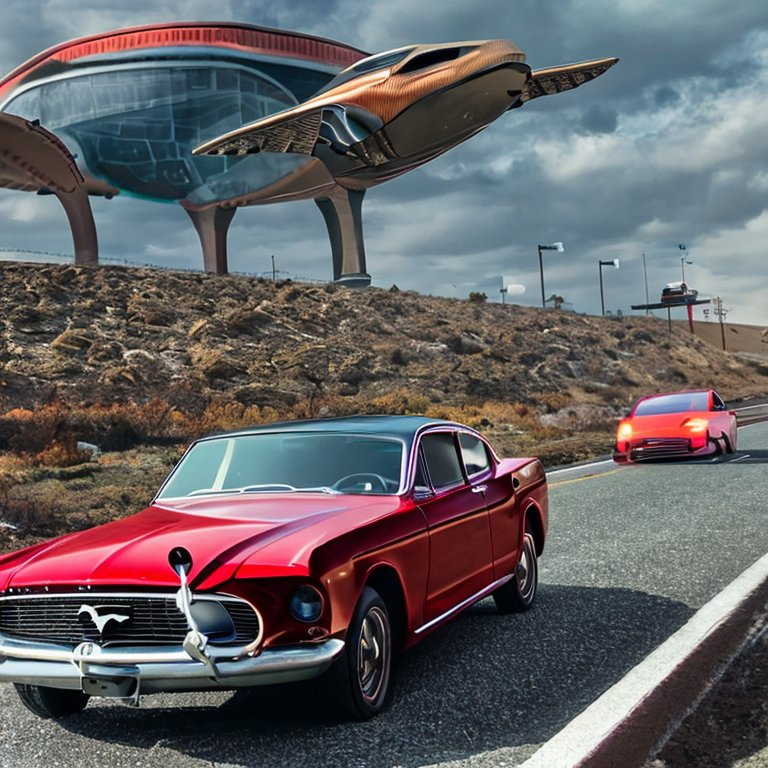
\includegraphics{mustang}
        \caption{"A steampunk scifi highway with a Tesla Model X driving next to a 1961 Ford Mustang" made with Stable Diffusion 2.1}
        \labfig{mustang}
\end{marginfigure}
\end{pdf}

Finally, communication is a vital aspect of autonomous driving infrastructure. Autonomous vehicles must be capable of communicating not only with other cars but also with people, animals, and various elements of the environment. The emergence of new technologies and trends, such as vehicle-to-vehicle (V2V) and vehicle-to-infrastructure (V2I) communication, has the potential to revolutionize the way self-driving cars interact with their surroundings. However, these advances also bring new challenges in terms of privacy, security, and standardization.

The development and adoption of autonomous vehicles are not solely dependent on the cars themselves but also on the supporting infrastructure. By addressing the challenges and seizing the opportunities presented by maps, roads, sensors, software, and communications, we can work toward a future where self-driving cars and human-driven vehicles coexist harmoniously within a dynamic, evolving transportation ecosystem.

\section{See You In Court!}

As autonomous vehicles become more prevalent, it is inevitable that their integration into society will bring legal challenges and disputes. In this section, we will examine the complexities of multicollinearity and mathematical chaos, explainability and accountability in court, and the role of trustworthy machine learning and inherently interpretable models in addressing these challenges.

Multicollinearity and mathematical chaos introduce an element of uncertainty in the performance of autonomous vehicles. As multiple, highly correlated variables affect the behavior of self-driving cars, determining the cause of a specific event can be difficult. This problem is exacerbated by the chaotic nature of the systems involved, where small changes in initial conditions can lead to vastly different outcomes. These factors can make it challenging to attribute responsibility in the event of an accident, particularly when attempting to disentangle the contributions of various components, such as hardware, software, and environmental factors.

\begin{pdf}
\begin{marginfigure}[-5.5cm]
        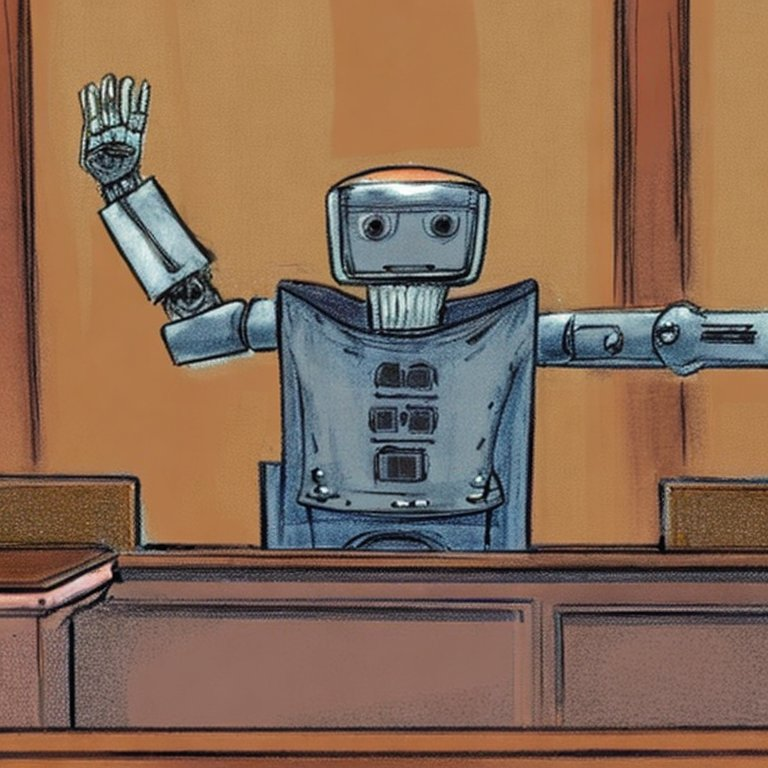
\includegraphics{robotcourt}
        \caption{"A courtroom sketch of a robot shrugging at the witness stand" made with Stable Diffusion 2.1}
        \labfig{robotcourt}
\end{marginfigure}
\end{pdf}

Explainability and accountability are critical concerns when presenting autonomous vehicle-related cases in court. If the decision-making processes of self-driving cars are inscrutable or difficult to understand, it becomes challenging to determine who or what is at fault in a given situation. This lack of transparency can impede the legal process and erode public trust in autonomous vehicle technology.

One potential solution to these challenges is the development of trustworthy machine learning, as described in Trustworthy ML\sidecite{trustworthyml}. By teaching developers to build models that are reliable, interpretable, and robust, we can create autonomous vehicles that are more easily understood and evaluated in legal proceedings. This approach prioritizes transparency and accountability, ensuring that the underlying algorithms driving these vehicles can be scrutinized and their decisions explained. 

In order to achieve explainability in artificial intelligence, it may be necessary to reconsider the recent advancements in deep neural networks. While these networks have demonstrated impressive performance, their opacity can make it difficult to understand how decisions are being made. This is where less advanced technology may have an advantage, as it allows for more transparency in the decision-making process. However, even with less advanced models such as decision trees, there is still the potential for complexity to create challenges in explainability. While theoretically fully explainable, decision trees can become cumbersome when they contain millions of lines of rules or code. As a result, they can be just as difficult to explain in a court of law as more advanced neural networks.

Inherently interpretable models further reinforce the case for transparency and accountability in autonomous vehicles. By developing machine learning models that are not only accurate but also readily interpretable, we can facilitate a more straightforward assessment of responsibility in the event of an accident. This clarity can help build public trust in the technology while also streamlining the legal process when disputes arise.

\section{Alternative Approaches}

As we explore the future of autonomous vehicles, it is crucial to consider alternative ways of thinking about self-driving cars and their potential roles in our transportation ecosystem. In this section, we will discuss various concepts that challenge conventional notions of autonomy and offer novel solutions that could complement or transform our understanding of mobility.

One alternative approach involves reimagining self-driving cars as a form of "train" that operates in dedicated lanes. By constructing special lanes for autonomous vehicles, we can essentially put these cars "on rails," enabling them to function more like a train. This approach would not only enhance the safety and efficiency of autonomous vehicles but also provide a glimpse into the potential infrastructural and regulatory frameworks necessary for their success.

In the realm of logistics and warehousing, the lack of self-driving forklifts offers an interesting lesson. Instead of focusing on automating forklifts, warehouses have implemented moving shelves, essentially flipping the problem on its head to achieve a more efficient solution. This example highlights the importance of rethinking traditional approaches to autonomy and searching for innovative ways to streamline various aspects of our economy.

\begin{pdf}
\begin{marginfigure}[-5.5cm]
        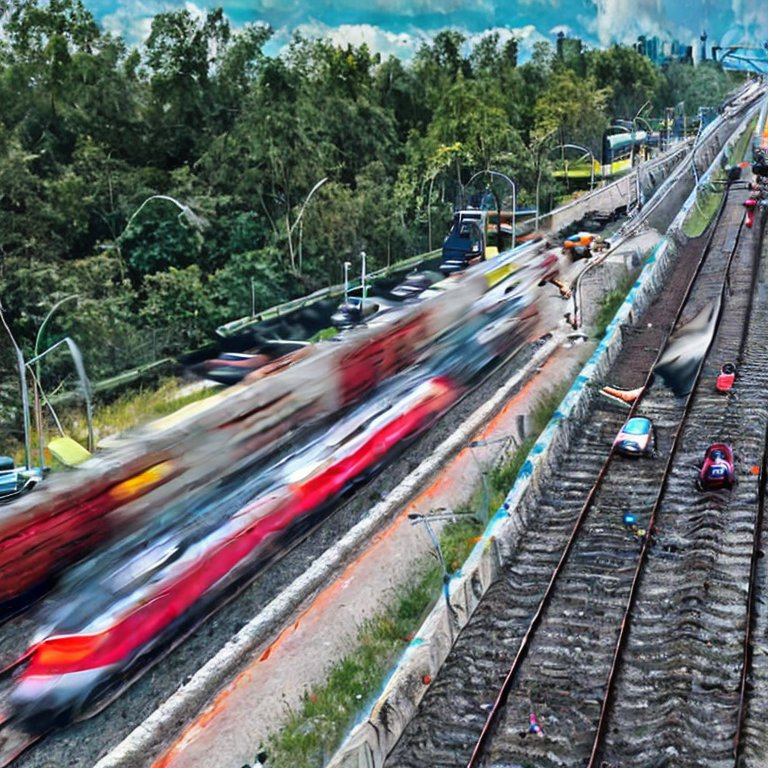
\includegraphics{trains}
        \caption{"trains going down the highway next to cars, bicycles and scooters" made with Stable Diffusion 2.1}
        \labfig{trains}
\end{marginfigure}
\end{pdf}

Building on these ideas, we can explore other unconventional approaches that challenge the status quo of autonomous vehicles. One possibility is the development of platooning systems, in which multiple vehicles travel in close proximity, communicating with one another to maintain safety and optimize traffic flow. This approach could harness the advantages of vehicle-to-vehicle communication while reducing the need for extensive infrastructure modifications.

Another alternative is the concept of supervised autonomy, not from the driver at a moment's notice like we have today, but from a control tower similar to those used at airports. This has large privacy implications but combines the benefits of autonomous technology with human oversight. This approach allows for human intervention in complex or high-risk situations, mitigating concerns about delegating life-or-death decisions to machines while still reaping the rewards of autonomous driving.

In all these alternative approaches, the key is to think creatively about how we can integrate self-driving cars into our transportation systems. By challenging conventional wisdom and exploring innovative solutions, we can create a more efficient, sustainable, and harmonious future for transportation, one that redefines the role of autonomous vehicles within an ever-evolving paradigm.

\section{Key Takeaways}

\begin{itemize}
\item \textbf{Redefine autonomy with alternative approaches:} Consider dedicated lanes, supervised autonomy, and other unconventional methods to enhance safety and efficiency while reimagining the role of self-driving cars in our transportation systems.
\item \textbf{Adapt to ever-changing driving infrastructure:} Address challenges in maps, roads, sensors, software, and communications to create a seamless, harmonious driving experience, while ensuring regular maintenance and updates. Embrace open-source software and standardized solutions to foster collaboration and innovation.
\item \textbf{Prioritize explainability and accountability:} Develop trustworthy machine learning and inherently interpretable models to enhance transparency, facilitate legal proceedings, and build public trust in autonomous vehicle technology.
\item \textbf{Leverage communication and collaboration:} Promote vehicle-to-vehicle communication, coordination with external systems, and remote control for improved safety, efficiency, and adaptability in a dynamic transportation environment. Encourage the adoption of industry standards to facilitate interoperability and streamline implementation.
\item \textbf{Balance innovation with regulation:} Establish robust regulatory frameworks that protect privacy, maintain accountability, and ensure safety while fostering technological advancements, and integrating autonomous vehicles into our evolving transportation landscape.
\end{itemize}
 
%\setchapterpreamble[u]{\margintoc}
\chapter{Revolutionary for Whom?}
\labch{rev}

\textit{"The inhabitant of London could order by telephone, sipping his morning tea in bed, the various products of the whole earth -- he could at the same time and by the same means adventure his wealth in the natural resources and new enterprise of any quarter of the world -- he could secure forthwith, if he wished, cheap and comfortable means of transit to any country or climate without passport or other formality."} John Maynard Keynes, 1920 \cite{Keynes2012}

\textit{"Living off the wits of his subordinates - maybe that's leadership these days" from Tinker, Tailor, Soldier, Spy by John Le Carre, 1974}\cite{Lecarre}

\section{The Battle of the Assistants}

Butler vs Indian Virtual Assistant vs Siri

Siri is hackable \url{https://arstechnica.com/information-technology/2023/02/ai-powered-bing-chat-spills-its-secrets-via-prompt-injection-attack/}

\section{Employees That Are Better Than You}

Respond directly to Jon Krohn's TED talk about monkeys being dumber than us... what about construction equipmenth that's stronger than us physically, or racism/eugenics people that are dumber than us \sidecite{KrohnTED}

\section{Slow on the Uptake}

\url{https://www.economist.com/finance-and-economics/2023/02/02/the-ai-boom-lessons-from-history} talk about historical perspective of technological change. Counter the narrative of "fastest tech to 1 million users" for ChatGPT.

\section{Free-Rider Problems}

I can steal your AI quite easily from outputs

Do we really need agreements like this? \url{https://www.reuters.com/technology/white-house-european-commission-launch-first-of-its-kind-ai-agreement-2023-01-27/}

The legal challenges are just beginning \url{https://techcrunch.com/2023/01/27/the-current-legal-cases-against-generative-ai-are-just-the-beginning/}.

\section{When You Can't Tell The Difference}

Talk about Taleb's aphorisms "Another definition of modernity: conversations can be more and more completely reconstructed with clips from other conversations taking place at the same time on the planet.", "You are alive in inverse proportion to the density of cliches in your writing."

Blurry JPEg of the web \url{https://www.newyorker.com/tech/annals-of-technology/chatgpt-is-a-blurry-jpeg-of-the-web}

\textit{"(Traditional) search engines are databases, organized collections of data that can be stored, updated, and retrieved at will. (Traditional) search engines are indexes. a form of database, that connect things like keywords to URLs; they can be swiftly updated, incrementally, bit by bit (as when you update a phone number in the database that holds your contacts).}

\textit{Large language models do something very different: they are not databases; they are text predictors, turbocharged versions of autocomplete. Fundamentally, what they learn are relationships between bits of text, like words, phrases, even whole sentences. And they use those relationships to predict other bits of text. And then they do something almost magical: they paraphrase those bits of texts, almost like a thesaurus but much much better. But as they do so, as they glom stuff together, something often gets lost in translation: which bits of text do and do not truly belong together."} Gary Marcus, 2023 \cite{marcus2023}


\section{Thinking Fast and Slow}

\textit{"The problem with the fast thinking is that it is often wrong. The problem with the slow thinking is that it is often too slow."} Daniel Kahneman, 2011 \cite{Kahneman2011}

\url{https://medium.com/@bitweis/why-chatgpt-fails-thinking-fast-and-slow-e3cdab18cd0}

\section{Dead Inside}

"If you know, in the morning, what your day looks like with any precision you are a little bit dead - the more precision the more dead you are."

\section{This Book is a Case Study}

Talk about "organic content" market.

\section{Managing Creative Destruction in Your Career}

\url{https://www.nist.gov/news-events/news/2023/01/nist-risk-management-framework-aims-improve-trustworthiness-artificial}

\url{https://learning.oreilly.com/library/view/manage-ai-bias/53863MIT64321/}

talk about how it changes careers.
 
%\setchapterpreamble[u]{\margintoc}
\chapter{Errors and Omissions}
\labch{intro}

 

%----------------------------------------------------------------------------------------

\backmatter % Denotes the end of the main document content
\setchapterstyle{plain} % Output plain chapters from this point onwards

%----------------------------------------------------------------------------------------
%	BIBLIOGRAPHY
%----------------------------------------------------------------------------------------

% The bibliography needs to be compiled with biber using your LaTeX editor, or on the command line with 'biber main' from the template directory

\defbibnote{bibnote}{Here are the references in citation order.\par\bigskip} % Prepend this text to the bibliography
\printbibliography[heading=bibintoc, title=Bibliography, prenote=bibnote] % Add the bibliography heading to the ToC, set the title of the bibliography and output the bibliography note

%----------------------------------------------------------------------------------------
%	BACK COVER
%----------------------------------------------------------------------------------------

% If you have a PDF/image file that you want to use as a back cover, uncomment the following lines

%\clearpage
%\thispagestyle{empty}
%\null%
%\clearpage
%\includepdf{cover-back.pdf}

%----------------------------------------------------------------------------------------

\end{document}
